%%%%%%%%%%%%%%%%%%%%%%%%%%%%%%%%%%%%%%%%%%%%%%%%%%%%%%%%%%%%%%%%%%%%%
%% Copyright 2020 Mike Jones, <dr.mike.jones@gmail.com>
%% AKA Grey Wolf <mike.jones@mansouthscouts.org>
%% [23rd Manchester (Birch with Fallowfield)]
%% Scout Membership number: 12114313
%
% This file is part of Grey Wolf's Scouts Beamer Theme.
%
% Grey Wolf's Scouts Beamer Theme is free software: you can redistribute
% it and/or modify it under the terms of the GNU General Public License
% as published by the Free Software Foundation, either version 3 of the
% License, or (at your option) any later version.
%
% Grey Wolf's Scouts Beamer Theme is distributed in the hope that it will 
% be useful, but WITHOUT ANY WARRANTY; without even the implied warranty
% of MERCHANTABILITY or FITNESS FOR A PARTICULAR PURPOSE.  See the GNU
% General Public License for more details.
%
% You should have received a copy of the GNU General Public License
% along with Grey Wolf's Scouts Beamer Theme.  If not, see
% <https://www.gnu.org/licenses/>.
%%%%%%%%%%%%%%%%%%%%%%%%%%%%%%%%%%%%%%%%%%%%%%%%%%%%%%%%%%%%%%%%%%%%%

\documentclass[aspectratio=169,utf8,t]{beamer}
% I've put some non-scout related preamble specific to this demo
% in the file oddsAndEnds.tex. For example code to markup bash scripts.
% Use listings for inclustion of code here I've setup basic shell script
\usepackage{listings} % A rich verbatum environment for code snippets
%\usepackage{fontawesome} % For funky symbols -- didn't use it in the end
\usepackage{multimedia} % Not sure how overleaf deals with this
\usepackage{grffile} % Fix Filename dummies thrown out of prams
\usepackage{tabularx,booktabs} % Use a richer tabular environment
\usepackage{lipsum}% Rhubarb rhubarb rhubarb. Saves having to type rhubard...

\usepackage{hologo}% Provides e.g. \pdfLaTeX
\usepackage{caption}% Better figure captioning

%We have arrows in the commands.tex slide deck
\usepackage{tikz}
\usetikzlibrary{arrows.meta,arrows}

%Adds a part page at \appendex command
\usepackage{appendix}

%References to footnotes
%https://tex.stackexchange.com/questions/16866/how-can-i-use-footnotemark-with-a-ref-argument
\usepackage{refcount}

%Suppress warnings when multiple PDFs with Page Groups are included on a single page
%https://tex.stackexchange.com/questions/76273/multiple-pdfs-with-page-group-included-in-a-single-page-warning#78020
\pdfsuppresswarningpagegroup=1

%Suppress syntax highlighting in comments of listing environments -- a hack
%https://tex.stackexchange.com/questions/378307/advanced-string-highlighting-in-listings#answer-378367
\def\bluecolorifnotalreadypurple{%
    \extractcolorspec{.}\currentcolor
    \extractcolorspec{purple}\stringcolor
    \ifx\currentcolor\stringcolor\else
        \color{blue}%
    \fi
}

%Colourize bash script highlighting in listing environments
\lstset{ 
  language=bash,
  showstringspaces=false,
  commentstyle=\color{red}, 
  keywordstyle=\bluecolorifnotalreadypurple,
  breaklines=true,
  breakatwhitespace=true,
% Can't have this next line in overleaf no colour allowed here!?
%  postbreak=\mbox{\textcolor{red}{$\hookrightarrow$}\space},
  postbreak=\mbox{$\hookrightarrow$\space},
  stringstyle=\color{purple},
  moredelim=[s][\color{purple}]'',
  morestring={**[s][\color{purple}]{<<'EOF'}{EOF}},
  morestring={**[s][\color{purple}]{<<EOF}{EOF}},
  basicstyle=\ttfamily,
  numbers=left,
  numberstyle=\tiny\color{gray}, % because america
  numbersep=5pt
}

% Patch Listing's line number to match lines of included section of file
%https://tex.stackexchange.com/questions/26828/first-line-number-in-lstinputlisting-environment#answer-27240
\makeatletter
\patchcmd{\lst@GLI@}% <command>
  {\def\lst@firstline{#1\relax}}% <search>
  {\def\lst@firstline{#1\relax}\def\lst@firstnumber{#1\relax}}% <replace>
  {\typeout{listings firstnumber=firstline}}% <success>
  {\typeout{listings firstnumber not set}}% <failure>
\makeatother

% In verbatum/lstlisting \end{frame} gets confused so can use \begin/end{slide} to safely encapsulate
% I inadvertently solved this by using lstinputlisting in a later revision, but leaving this in in case.
% https://tex.stackexchange.com/questions/467672/problems-with-fragile-frames-in-beamer#467675
\newenvironment{slide}{\begin{frame}[fragile,environment=slide]}{\end{frame}}

% Start the footnotemarks at 2 for each new page
%\usepackage{perpage}
%\MakePerPage[2]{footnote} % I prefer a dagger.
%This sometimes causes "! LaTeX Error: Counter too large."
%Solution: use a better per page hook
%https://tex.stackexchange.com/questions/306396/paracol-how-to-reset-footnote-counter-every-page#306405
\usepackage{everypage}
\AddEverypageHook{\setcounter{footnote}{1}} % resets footnote counter on every page

% Use Symbols in footnotes
\renewcommand{\thefootnote}{\fnsymbol{footnote}}



\usetheme{scouts}% Grey Wolf's Scouts Beamer Theme creates by Mike Jones

% The optional `\author` macro defines the author and is displayed
% in the slide produced by the `\titlepage` command.
\author{Grey Wolf}

% The optional `\institute` macro defines the author and is displayed
% in the slide produced by the `\titlepage` command. It also provides
% the default text for the macro \logoslide.
\institute{\href{https://mansouthscouts.org.uk/our-groups/23rdManchester}{23rd~Manchester}
\\\href{https://mansouthscouts.org.uk/our-groups/23rdManchester}{(Birch~with~Fallowfield)}}

% The optional `\title` macro defines the title and is displayed
% in the slide produced by the `\titlepage` command. The '\title'
% will be shown in the headline at the top left of all other slides
% unless disabled by the \NNNNNN macro.
\title{Do~more. Share~more. Be~more.}

% The '\subtitle' macro, if specified, will add a smaller subtitle 
% below the main one, and will not be displayed in any of the other slides.
% NB this additional to and not in the published Scouts PPT Template
%\subtitle{Subtitle goes here if needed}

% Optional `\date` macro will display a custom free text date on the
% all of the slides' footer. If omitted today's date will be used.
%\date{2020-07-25}


\begin{document}
\headervisibility[combined,hidepartnum]
\logoslide[noheadlogo]

\begin{frame}
\begin{abstract}
What follows is a test, a demonstration, an exploration and some documentation about how this Beamer template/theme.  It is split into separate parts (listed below) and covers why I created this theme,\footnote{In \LaTeX{}'s Beamer document class, a theme is essentially a template.} how to use it, a reproduction of the Scout Branding Centre's Powerpoint slides, some test slides and an example walkthrough from the Beamer documentation.
\end{abstract}
\end{frame}

\frame{\frametitle{What's Coming up...}\tableofcontents[onlyparts]}

\title{Do~more. Share~more. Be~more.}
\part{How did this template come about?}
%%%%%%%%%%%%%%%%%%%%%%%%%%%%%%%%%%%%%%%%%%%%%%%%%%%%%%%%%%%%%%%%%%%%%
%% Copyright 2020 Mike Jones, <dr.mike.jones@gmail.com>
%% AKA Grey Wolf <mike.jones@mansouthscouts.org>
%% [23rd Manchester (Birch with Fallowfield)]
%% Scout Membership number: 12114313
%
% This file is part of Grey Wolf's Scouts Beamer Theme.
%
% Grey Wolf's Scouts Beamer Theme is free software: you can redistribute
% it and/or modify it under the terms of the GNU General Public License
% as published by the Free Software Foundation, either version 3 of the
% License, or (at your option) any later version.
%
% Grey Wolf's Scouts Beamer Theme is distributed in the hope that it will 
% be useful, but WITHOUT ANY WARRANTY; without even the implied warranty
% of MERCHANTABILITY or FITNESS FOR A PARTICULAR PURPOSE.  See the GNU
% General Public License for more details.
%
% You should have received a copy of the GNU General Public License
% along with Grey Wolf's Scouts Beamer Theme.  If not, see
% <https://www.gnu.org/licenses/>.
%%%%%%%%%%%%%%%%%%%%%%%%%%%%%%%%%%%%%%%%%%%%%%%%%%%%%%%%%%%%%%%%%%%%%

\changecolours{ScoutPurple}
\section*{Why a \LaTeX{} Beamer theme}
\subsection{Just prep for another all section Scout Meeting}

\frame{
This is the story about how this Scouts Beamer template came into existance.
In what follows, you'll find pictures, anicdotes, wild assertions, not a small amount of computing code and, I fancy, an embedded media file\footnote{You'll need a PDF reader that understands ``embedded'' \emph{rich} media (Adobe Reader v9+ and Okular v0.15+.  You'll also need the embedded media alongside, 'cause it's not really embedded is it!}
}

{
\setbeamerfont{footnote}{size=\Tiny}
\frame{
\frametitle{We had a Leaders' planning meeting over Zoom.}
\scriptsize How do we startup after a (very) extended Easter break?
\vspace{-3mm}
\begin{figure}
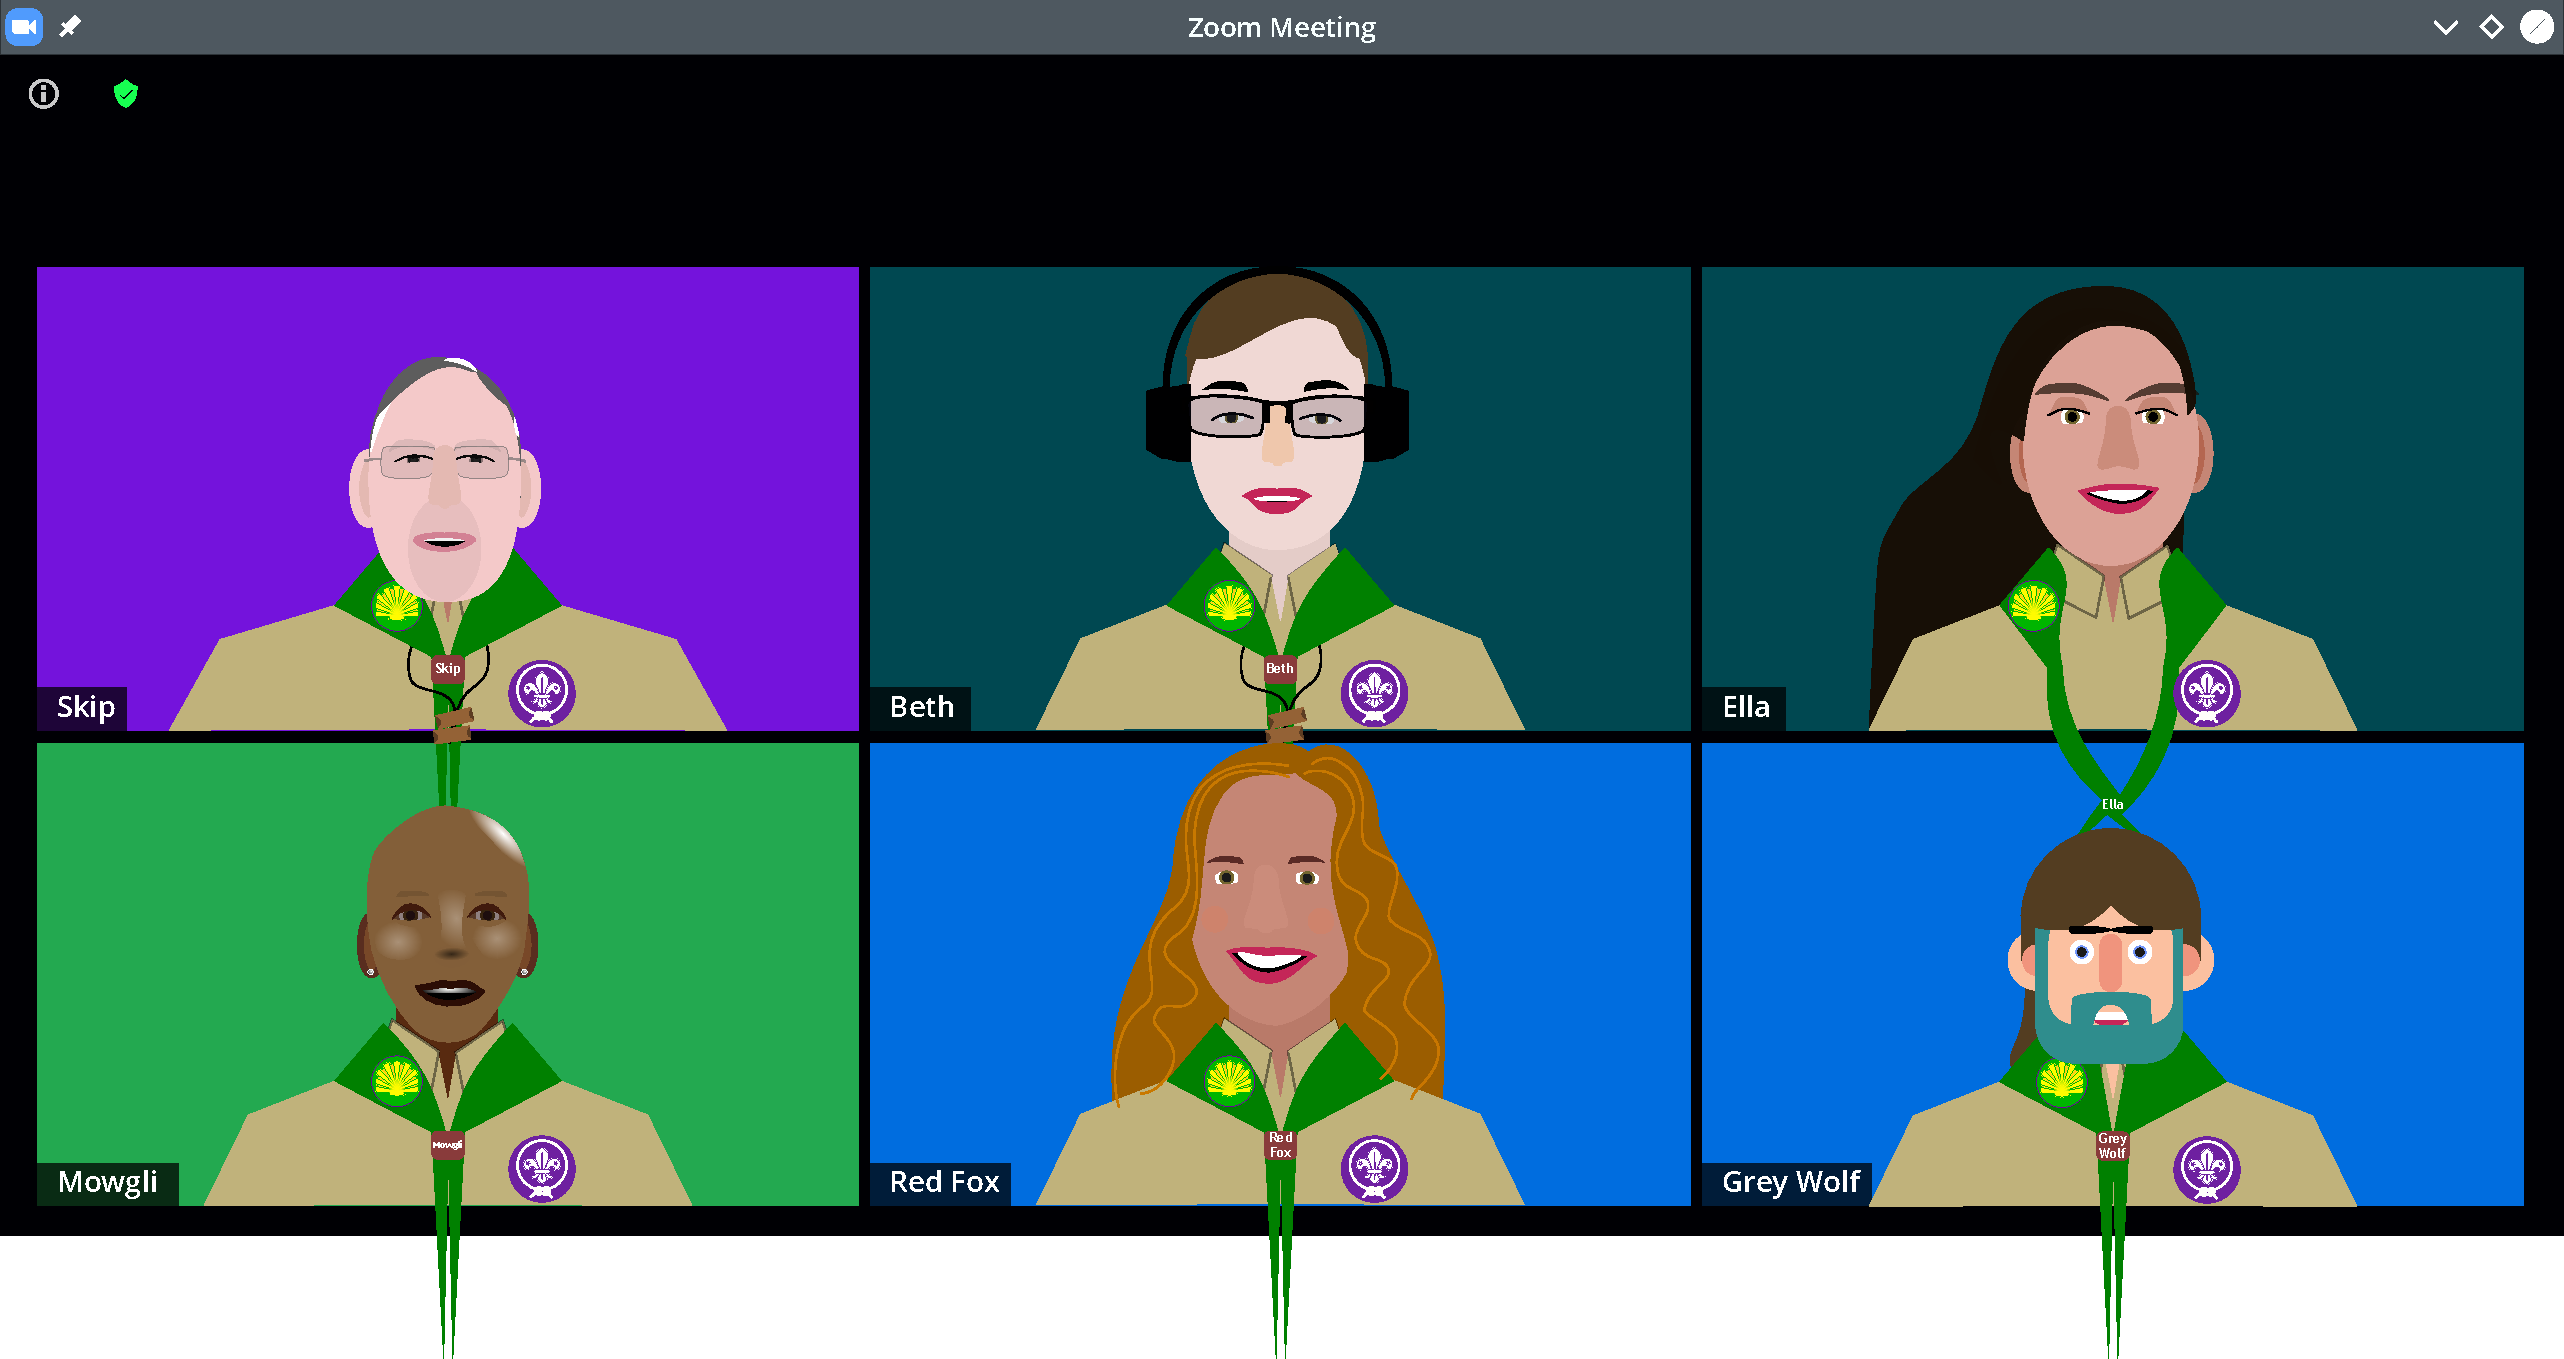
\includegraphics[height=0.7\textheight,keepaspectratio]{Motivation/images/zoom}
\vspace{-5mm}
\caption{The actual\footnote{We did have a zoom meeting but it didn't look quite like this.} zoom meeting.}
\end{figure}
\vspace{-2mm}
}
}

{
\changecolours[inverse]{ScoutYellow}
\headervisibility[hideheadlogo]
\bgimage[position=r,gravity=E,fit=height]{Motivation/images/CoronaDoLess.pdf}
\twocolframe[leftcol=7cm,rightcol=3cm]{%
\Large There was\footnote[frame]{is---at time of writing.} a pandemic going on don't you know!

\vspace{0.5\baselineskip}
With no meetings, I for one was stuck inside with little more to keep me out of trouble than generating sick memes.

\vspace{0.5\baselineskip}
What \alert{were} our YMs doing?}{}
}

{
\changecolours[inverse]{ScoutBlue}
\bgimage[position=l,gravity=C]{Motivation/images/Okay.jpg}
\twocolframe{}{\large District was encouraging us to hold some kind of sessions for the wellbeing of the young members.
\par\vspace{\baselineskip}
\alert{But what could we do?}
}
}

{
\changecolours[inverse]{ScoutGreen}
\bgimage[position=l,gravity=W]{Motivation/images/cycling1}
\twocolframe[titleright={Cycling badge}]{}{%
I'd noticed many of our young members and their families taking to their bicycles for their daily exercise.

\par\vspace{\baselineskip}
I thought we could use this to drive through the Cyclist Activity badges across the various sections.
}
}

\frame{
\frametitle{So a Quiz! Quizzes work online, right?}
Road safety and the use of roads is part of cycling.

And in Manchester we have:
\itemseps[topsepi=0.5mm,itemsepi=0.5mm]
\begin{itemize}
\item a lot of roads,
\item a lot of tow paths (some accessable to bikes),
\item a lot of dedicated and shared bike lanes,
\item and lots of National Cycle Network routes.
\end{itemize}
How about a multiple guess quiz on some of our UK signage.
}

{
\changecolours[inverse]{ScoutBlack}
\headervisibility[hideheadtext]
\bgimage[position=f,gravity=C,fit=all,transparency=0.7,ignoreaspectratio]{Motivation/images/GSLs.jpg}
\frame{
\frametitle{Also happening at the same time...}
Scout HQ has been working on rebranding, and \mbox{23\raisebox{0.6ex}{\scriptsize rd} Manchester} has been working as a group to overhaul our web presence.
\par%\vspace{\baselineskip}
I thought well, can't I just use something from the Scout Brand Centre?
}
}

\frame{
\frametitle{Getting the information}
\begin{itemize}
\item I found the UK government road sign website: \href{https://www.gov.uk/guidance/traffic-sign-images}{https://www.gov.uk/guidance/traffic-sign-images}. This had
\begin{itemize}
\item zip files of all the signs graphics.
\item a spreadsheet describing the road signs.
\end{itemize}
\item All I needed now was a way to make this into an online multiple choice quiz.
\end{itemize}
}

\frame{
\frametitle{Automation}
Having identified 25 road signs that I could work with I now had the task of importing and resizing 25 images, formatting slides, and adding 25 captions.
\par%\vspace{\baselineskip}
But \alert{What are computers for?} ...if not to make repetitive and time consuming tasks easy?
}

\frame{
\frametitle{Automation}
\itemseps[topsepi=0mm,itemsepi=0mm]
\begin{enumerate} 
\item I considered writing a script to create slides using one of the PPTX APIs. 
\item I also considered copying the template to Google Sheets and writing a Google App script\footnote{I'm more familiar with GoogleDocs. Moreover, I don't have Microsoft at home and the O365 PowerPoint landscape is IMHO a buggy and featureless terrain.} 
\end{enumerate}
\parbox{\textwidth}{I'm also more at home with \href{https://www.fsf.org/}{Free and Open Source Software}, how about something like \href{https://www.libreoffice.org/}{LibreOffice}?}
}

\frame{
\frametitle{How about \LaTeX}
I'd worked with \LaTeX{} before, in the world of academia. 
I had used it to write letters, articles and documents
and occasionally the odd slide deck for work.
This would be a bit different though, \LaTeX{} is a typesetting tool.
In my experience good for scientific papers and simple non-glossy stuff.
}

\subsection{Creating the slides}

\begin{frame}[fragile]{But...}
It is kind of easy to write slides, once there's a template. 
For example, here is the \emph{code} for the last two slides:
\tiny
\begin{verbatim}
\frame{
\frametitle{How about \LaTeX}
I'd worked with \LaTeX before, in the world of academia.
I had used it to write letters, articles and documents
and occasionally the odd slide deck for work.
This would be a bit different though, \LaTeX is a typesetting tool.
In my expreience good for scientific papers and simple non-glossy stuff.
}
\subsection{Creating the slides}
\end{verbatim}
\end{frame}

\section*{Lets look at the code.}

\subsection{The following section is probably not for the faint hearted.}

{
\setbeamerfont{footnote}{size=\Tiny}
\begin{frame}{Here comes a bash script to make us some slides}
\footnotesize
\parbox{\textwidth}{\alert{And before you ask...} No! I didn't write the following script then execute it like some kind of crazy robot. I did this one step at a time, bit--by--bit over the course of about an hour\textsuperscript{TM\footnote{For large values of one hour\textsuperscript{TM}.}}.}

\parbox{\textwidth}{I searched the web; found the stuff; converted the format of the long list from the web; downloaded the images; made a short list of signs I liked; \href{https://en.wikipedia.org/wiki/Grep}{grep}ped\footnote{\tt grep, egrep, fgrep, rgrep - print lines matching a pattern} the signs I liked into a loop where I converted my favourite signs to pdf and with a \LaTeX{} template spat out the file: {\tt include.tex}. Then I merged that file into my scoutified CERN Beamer template.  What follows is what you might get if you crush all that work into a hairy \href{https://www.gnu.org/software/bash/}{bash} script.
\hfill
\hyperlink{quizslides}{\beamerskipbutton{skip}}
}
\end{frame}
}

\begin{frame}{Breakdown of bash script to make the quiz skeleton slides...}
\parbox{\textwidth}{Lets start by getting the {\tt Beamer} template\footnote{At the time of writing this template is only available to me in my \href{https://www.overleaf.com/project/5f1c704829d3e800016ed5c3}{overleaf.com} account and private \href{https://github.com/nimpo/GreyWolfsScoutsBeamerTheme}{github.com} repo.}. I started with a Scouty tweak to the \href{https://www.overleaf.com/latex/templates/cern-presentation-title/mgnwzmtgtvkw}{CERN Presentation template} by J\'er\^ome Belleman, but the git repository in the listing now holds the template used for this presentation:}
\tiny
\end{frame}

\begin{frame}{Breakdown of bash script (continued)...}
\parbox{\textwidth}{\small I searched the web; found the UK Government's \href{https://www.gov.uk/guidance/traffic-sign-images}{traffic sign images} webpage. The following snippet (lines 6--14) screen-scrapes the site and downloads\footnote{Here I used \href{https://curl.haxx.se/}{curl}.} the Excel file with all the road sign descriptions:}
\tiny
\lstinputlisting[firstline=6,lastline=14]{Motivation/quizscript.sh}
\end{frame}

\begin{frame}{Breakdown of bash script (continued)...}
\parbox{\textwidth}{\small I used \href{https://www.libreoffice.org/}{LibreOffice} to convert the MS Excel document to something a bit more universal and which we can work with. Here, in the script, a sleepy loop is required here because LibreOffice runs this command asynchronously:}
\tiny
\lstinputlisting[firstline=16,lastline=23]{Motivation/quizscript.sh}
\end{frame}


\begin{frame}{Breakdown of bash script (continued)...}
\parbox{\textwidth}{We need columns 12 and 3\footnote{The filename for the encapsulated postscript version of the sign, and its ``Caption''} from the CSV file. I've used the handy tool called \href{https://packages.ubuntu.com/bionic/csvtool}{\tt csvtool}. The results will be TAB separated and saved into a {\tt .tsv} file.}
\tiny
\lstinputlisting[firstline=25,lastline=26]{Motivation/quizscript.sh}
\end{frame}

\begin{frame}{Breakdown of bash script (continued)...}
\parbox{\textwidth}{\small Screen-scraping the \href{https://www.gov.uk/guidance/traffic-sign-images}{gov.uk} site again we download all the signs in eps\footnote{Encapsulated postscript is widely supported vector format often used in the printing industry.} format in their zipped bundles. We'll get each zip file and unzip it into the directory {\tt SignsDL} for later.}
\tiny
\lstinputlisting[firstline=28,lastline=35]{Motivation/quizscript.sh}
\end{frame}

\section*{Take a break here.}
\subsection{...and make some coffee. That's what I did.}
\section*{Lets look at the code.}
\setlength{\fboxsep}{0pt}
\begin{frame}{Breakdown of bash script (continued)...}
\parbox{\textwidth}{\small Coffee in hand, have a look through the signs and choose some nice ones. I chose these...}

\parbox[c]{0.07\textwidth}{%
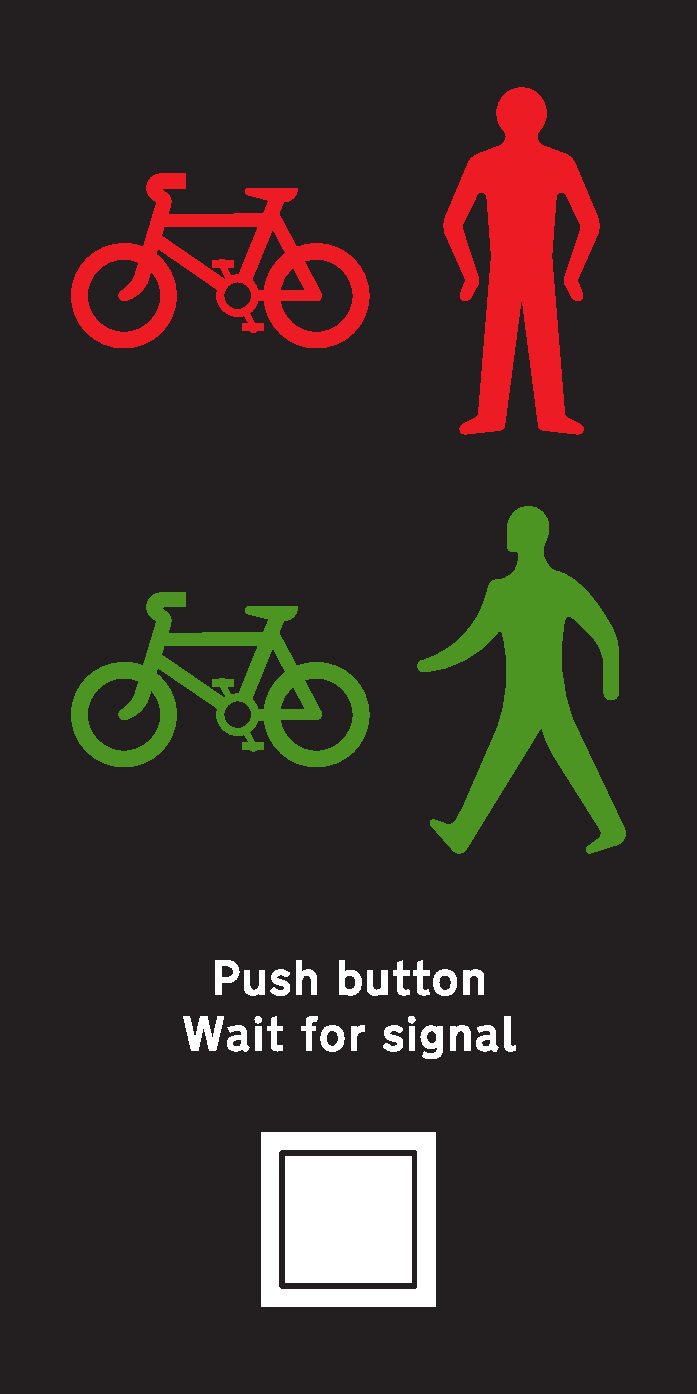
\includegraphics[width=0.06\textwidth]{Motivation/Signs/4003.7}}%
\parbox[c]{0.93\textwidth}{\raggedright

\includegraphics[width=0.06\textwidth]{Motivation/Signs/2602.2}

\includegraphics[width=0.06\textwidth]{Motivation/Signs/2603}

\includegraphics[width=0.06\textwidth]{Motivation/Signs/2702}

\includegraphics[width=0.06\textwidth]{Motivation/Signs/2928}

\includegraphics[width=0.06\textwidth]{Motivation/Signs/501}

\includegraphics[width=0.06\textwidth]{Motivation/Signs/512}

\includegraphics[width=0.06\textwidth]{Motivation/Signs/520}

\includegraphics[width=0.06\textwidth]{Motivation/Signs/522}
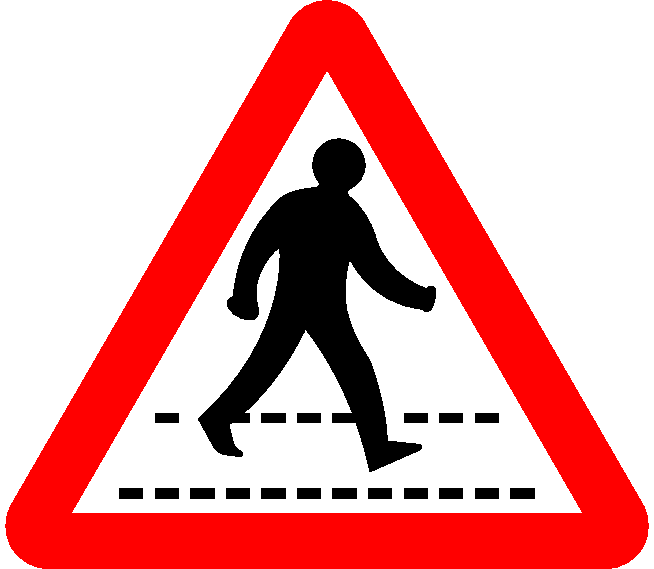
\includegraphics[width=0.06\textwidth]{Motivation/Signs/544}

\includegraphics[width=0.06\textwidth]{Motivation/Signs/551.2}
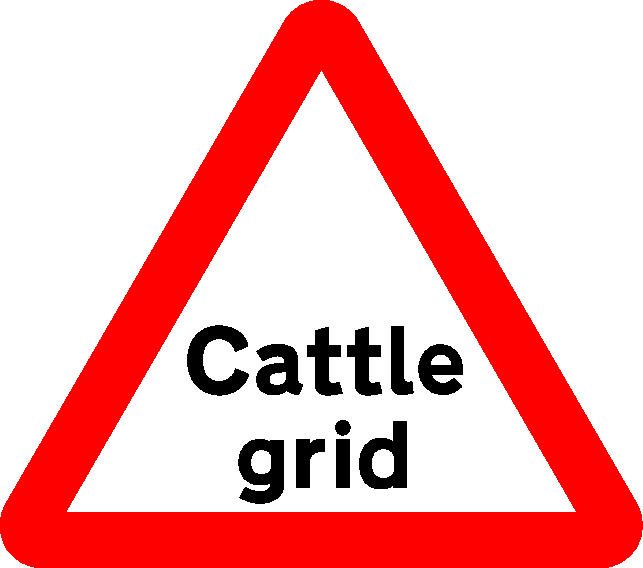
\includegraphics[width=0.06\textwidth]{Motivation/Signs/552}

\includegraphics[width=0.06\textwidth]{Motivation/Signs/555}

\includegraphics[width=0.06\textwidth]{Motivation/Signs/562}

\includegraphics[width=0.06\textwidth]{Motivation/Signs/670V20}

\includegraphics[width=0.06\textwidth]{Motivation/Signs/7001}

\includegraphics[width=0.06\textwidth]{Motivation/Signs/770}

\includegraphics[width=0.06\textwidth]{Motivation/Signs/810}

\includegraphics[width=0.06\textwidth]{Motivation/Signs/827.2}

\includegraphics[width=0.06\textwidth]{Motivation/Signs/833}

\includegraphics[width=0.06\textwidth]{Motivation/Signs/834}

\includegraphics[width=0.06\textwidth]{Motivation/Signs/950}

\includegraphics[width=0.06\textwidth]{Motivation/Signs/951}

\includegraphics[width=0.06\textwidth]{Motivation/Signs/953.1V}

\includegraphics[width=0.06\textwidth]{Motivation/Signs/956}
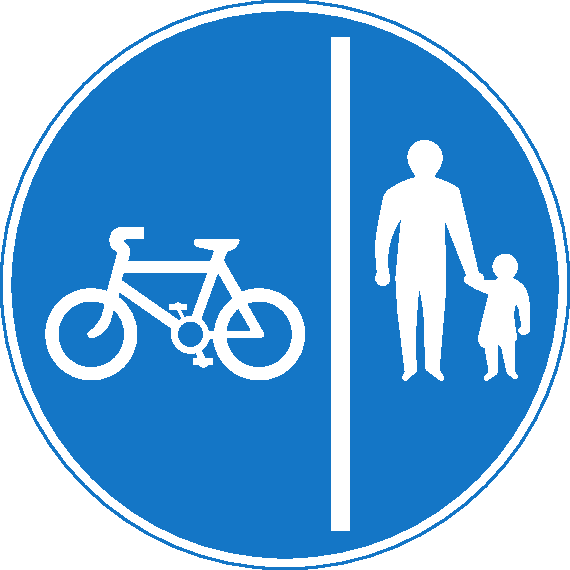
\includegraphics[width=0.06\textwidth]{Motivation/Signs/957}

\includegraphics[width=0.06\textwidth]{Motivation/Signs/T201}
}

\parbox{\textwidth}{\small Then in my script I set a variable to hold the label for each:}

\tiny
\lstinputlisting[firstline=37,lastline=38]{Motivation/quizscript.sh}
\end{frame}

\begin{frame}{Breakdown of bash script (continued)...}
\parbox{\textwidth}{Convert the nice ones into a format we can use\footnote{Encapsulated Postscript is fine for \LaTeX{} but is often in a CMYK colourspace. We want an RGB colourspace for screens (not print), and since I'm using \hologo{pdfLaTeX} I'll convert to PDF format.}. \href{https://inkscape.org/}{Inkscape} can do this in batchmode.}
\tiny
\lstinputlisting[firstline=40,lastline=49]{Motivation/quizscript.sh}
\end{frame}

\begin{frame}{Breakdown of bash script (continued)...}
The next\footnote{Next but one.} slide shows how to make the slide template. (It needs a slide all to itself.)

The resulting template will be used like a \href{https://en.wikipedia.org/wiki/Mail_merge}{mail merge}. However, instead of creating a letter template to later \emph{merge} with a database of multiple customers' details, we've got a slide template, multiple sign images and a look up table for each sign's corresponding captions.
\end{frame}

{
\changecolours{ScoutPink}
\bgimage[gravity=C,position=r]{Motivation/images/cat.jpg}
\twocolframe{Oh and the {\tt cat} you're about to see isn't grumpy.\par It just means spit the following stuff out ( and the '>' sends it to a file).}{}
}

\begin{frame}
\tiny
\lstinputlisting[firstline=51,lastline=74]{Motivation/quizscript.sh}
\end{frame}

\begin{frame}{Breakdown of bash script (continued)...}
\footnotesize Now we do the \emph{mail merge}--esque bit, looping over the {\tt \$SIGNS} we chose earlier. Line 77 just empties the file {\tt include.tex}. Then in a loop (78--83), I've used \href{https://en.wikipedia.org/wiki/AWK}{\tt awk} to extract each caption from the tsv file. Then using \href{https://en.wikipedia.org/wiki/Sed}{\tt sed}, we place the sign in the template's @LBL@ placeholder and then the real caption in a random position in the enumerated list e.g. @1@ to form one answer of the multiple guess.
\tiny
\lstinputlisting[firstline=76,lastline=83]{Motivation/quizscript.sh}
\end{frame}

\begin{frame}{Breakdown of bash script (continued)...}
\parbox{\textwidth}{\small The next slide shows how to make {\tt main.tex}, the primary file in the creation of the slides. Here's an overview:}

\small
\begin{description}[lines 96--103]
\item[line 90] Select the \href{https://ctan.org/pkg/beamer}{Beamer} document class.
\item[line 91] Select my ``scouts'' theme
\item[lines 92--95] Give \LaTeX{} the author and other {\tt \textbackslash{}titlepage} info
\item[lines 96--103] Holds the actual content of the slides.
\begin{description}[103,104]
\item[98] The title page slide
\item[100] Hwew we include the content from {\tt include.tex}
\item[101,102] Trailing slides: thank you and copyright notice.
\end{description}
\end{description}
\end{frame}

\begin{frame}{Breakdown of bash script (continued)...}
\tiny
\lstinputlisting[firstline=88,lastline=104]{Motivation/quizscript.sh}
\end{frame}

\begin{frame}{Compile it!}
Now all that's left to do is edit {\tt include.tex} to add the alternative answers to each slide/frame and any final tweaks. (I added two other versions of the county boundary signs and changed the NCN route from 14 to route 66.)
\begin{center}
\parbox{0.1\textwidth}{
\raggedleft
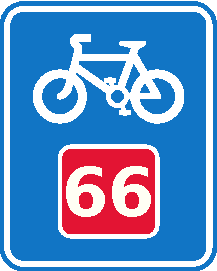
\includegraphics[width=0.1\textwidth]{Motivation/Signs/extra/2602.2-66}
}
\parbox{0.2\textwidth}{%
\centering%

\includegraphics[width=0.2\textwidth]{Motivation/Signs/2928}\\

\includegraphics[width=0.2\textwidth]{Motivation/Signs/extra/2928b}\\

\includegraphics[width=0.14\textwidth]{Motivation/Signs/extra/2928c}
}
\end{center}

Finally compile the code with: {\tt latexmk} and out should pop a main.pdf
\end{frame}

{
\setbeamerfont{footnote}{size=\Tiny}
\begin{frame}[label=quizslides]
\small
Here's an animation\footnote{The PDF reader needs access to the media file.} of the slideshow as it was:
\begin{center}
\movie[width=0.5\textwidth]{
\includegraphics[width=0.5\textwidth]{Motivation/movies/HighwayCode.png}\hspace{-0.48\textwidth}\raisebox{\depth}{Click image to start}}{Motivation/movies/HighwayCode.mp4}
\end{center}
You'll perhaps notice that the template I used in those slides was slightly different to this presentation.
\end{frame}
}

{
\setbeamerfont{footnote}{size=\Tiny}
\begin{frame}
\scriptsize
For completeness here's an animation of what all that scripting stuff above now spits out:
\begin{center}
\movie[width=0.5\textwidth]{
\includegraphics[width=0.5\textwidth]{Motivation/movies/HighwayCodeBikeQuizScripted.png}\hspace{-0.48\textwidth}\raisebox{\depth}{Click image to start}}{Motivation/movies/HighwayCodeBikeQuizScripted.mp4}
\end{center}
And that's what the template it looks like at the time of writing. 

With a couple of tweaks for example using the {\tt \textbackslash{}bgcolor} and {\tt \textbackslash{}twocolframe} macros the presentaion might look a bit like the one in \hyperlink{Part6}{\color{ScoutPurple}the appendix}.

The scripts can be found bundled with this theme: \href{file:Motivation/quizscript.sh}{\tt ./Motivation/quizscript.sh} and the modified updated one \href{file:Motivation/quizscript2.sh}{\tt ./Motivation/quizscript2.sh}.
\end{frame}
}


\changecolours{ScoutPurple}
\title{Code more. Share~more. Free~software.} 
\part{Using the theme}
%%%%%%%%%%%%%%%%%%%%%%%%%%%%%%%%%%%%%%%%%%%%%%%%%%%%%%%%%%%%%%%%%%%%%
%% Copyright 2020 Mike Jones, <dr.mike.jones@gmail.com>
%% AKA Grey Wolf <mike.jones@mansouthscouts.org>
%% [23rd Manchester (Birch with Fallowfield)]
%% Scout Membership number: 12114313
%
% This file is part of Grey Wolf's Scouts Beamer Theme.
%
% Grey Wolf's Scouts Beamer Theme is free software: you can redistribute
% it and/or modify it under the terms of the GNU General Public License
% as published by the Free Software Foundation, either version 3 of the
% License, or (at your option) any later version.
%
% Grey Wolf's Scouts Beamer Theme is distributed in the hope that it will 
% be useful, but WITHOUT ANY WARRANTY; without even the implied warranty
% of MERCHANTABILITY or FITNESS FOR A PARTICULAR PURPOSE.  See the GNU
% General Public License for more details.
%
% You should have received a copy of the GNU General Public License
% along with Grey Wolf's Scouts Beamer Theme.  If not, see
% <https://www.gnu.org/licenses/>.
%%%%%%%%%%%%%%%%%%%%%%%%%%%%%%%%%%%%%%%%%%%%%%%%%%%%%%%%%%%%%%%%%%%%%

\section{About this template}
\begin{frame}{About this template}
\parbox{\textwidth}{This theme is called \alert{Grey Wolf's Scouts Beamer Theme}.
It was created as a follow up to a quickly, thrown--together, slideshow--based quiz for our local scout group's Zoom session during the pandemic of 2020.}

\parbox{\textwidth}{The theme attempts to replicate the \href{https://scoutsbrand.org.uk/}{Scout Brand Centre}'s PowerPoint template using something called \href{https://www.latex-project.org/}{\LaTeX{}}.}
\end{frame}

{
\setbeamerfont{footnote}{size=\Tiny}
\begin{frame}{Your licence to use this theme.}
\tiny
\parbox{\textwidth}{\LaTeX{} is \href{https://www.debian.org/intro/free}{free software}.
It is licensed under \href{https://www.latex-project.org/lppl/}{LaTeX Project Public License} licence (LPPL). 
Many documents, 
\href{https://www.overleaf.com/gallery/tagged/presentation}{templates}, 
\href{http://www.texfaq.org/FAQ-clsvpkg}{styles/packages}, 
\href{http://www.texfaq.org/FAQ-clsvpkg}{classes} and 
\href{http://tug.ctan.org/macros/latex/contrib/beamer/doc/beameruserguide.pdf\#section.15}{beamer themes} 
written for \LaTeX{} are released under free software licences like the LPPL or \href{https://www.gnu.org/licenses/gpl-3.0.en.html}{GPL}; much of the content is released under one or other of the \href{https://creativecommons.org/}{Creative Commons licences}.}
 
\parbox{\textwidth}{The code I have written for the \alert{Grey Wolf's Scouts Beamer Theme} is hereby released under the GPLv3 licence (you are free to use any of my code provided here under the terms of that licence or any later version of the GPL at your descretion).
Other components of this theme not written by me---for example, those provided by the \href{https://scoutsbrand.org.uk/}{Scout Brand Centre}---or derived from other free software---for example, the \hyperlink{font}{OS2v3 version of the Nunito Sans font}---carry their own copyright and licence terms.\footnote{See the theme's accompanying \href{file:LICENCE}{\tt LICENCE} and \href{file:README.md}{\tt README.md} files.}}

\parbox{\textwidth}{Presentations consisting of your content and compiled with this theme are yours. The licences are concerened with the subsequent distribution of this software. The Scout Association's trademarks must however only be used in accordance with The Scout Association's regulations.}

\parbox{\textwidth}{What follows are a few slides describing this theme and how to use it.}
\end{frame}
}

\begin{frame}{The Font}
\hypertarget{font}{}
\small
\parbox{\textwidth}{This theme contains a copy of the
\href{https://fonts.google.com/specimen/Nunito+Sans}{Nunito-Sans}~font. 
I have had to make modifications to its encoding to enable
it to work in \LaTeX{}.
This means the TrueType (TTF) files referenced by the template are not the original Nunito-Sans TTF files.
There are few practical differences. However, to satisfy the Licence conditions of the font I have called the resulting font NunitoSansOS2v3 to distingush it as a derivative. Details are in the accompanying \href{file:texmf/fonts/truetype/NunitoSans/OS2v3/README.md}{\tt README.md} file. }

\parbox{\textwidth}{You can find the font and accompanying files in the \href{file:texmf/fonts/}{\tt texmf/fonts/}
and \href{file:texmf/tex/latex/psnfss/}{\tt texmf/tex/latex/psnfss/} directories.}
\end{frame}

\begin{frame}{Scout Brand Images}
\hypertarget{brand}{}
\scriptsize
\parbox{\textwidth}{The scout brand images were obtained from the \href{https://scoutsbrand.org.uk/}{Scout Brand Centre} website under licence. The Scout brand images are registered trademarks\footnote{See the corresponding entry registered with the UK Intellectual Property Office: \href{https://trademarks.ipo.gov.uk/ipo-tmcase/page/Results/1/UK00003310891}{UK00003310891}} and their use is further governed by Scouting policy.\footnote{See Protected Scout logos, names, badges and awards: \href{https://www.scouts.org.uk/por/14-other-matters/rule-147-protected-scout-logos-names-badges-and-awards/}{POR 147}}}

\parbox{\textwidth}{Where possible I prefer to use vector graphics. The Scout Brand Centre provides various formats for the various logos. Some have margins; some are without margins. For consistany I have converted these into PDF files with RGB colourspace and without borders/margins. I rely on the theme to place the images at their correct location with suitable margins.}

\parbox{\textwidth}{The brand related files are located in \href{file:texmf/tex/generic/images/Branding/}{\tt ./texmf/tex/generic/images/Branding/}}
\end{frame}

\begin{frame}{The Grey Wolf's Scout Beamer Theme files}
\scriptsize
\parbox{\textwidth}{In the remainder of this theme you'll find the usual \alert{beamertheme}: font, color, inner and outer {\tt .sty} files such as you might expect. You'll also find some \alert{beamerscouts} {\tt .sty} files which contain the various macros defined for the operation of the theme.}

\parbox{\textwidth}{The Scout Branding PowerPoint template does not separate well into the inner and outer components like a normal a Beamer theme. Inner and outer themes, although present, may not work as expected. As such you should not assume that it will be possible to mix with other Beamer themes.}

\parbox{\textwidth}{You enable this theme by adding the following line to your Beamer document's preamble: \alert{{\tt \textbackslash{}usetheme\{scouts\}}}. This loads {\tt beamercolorthemescouts.sty}, {\tt beamerfontthemescouts.sty}, {\tt beamerinnerthemescouts.sty} and {\tt beamerouterthemescouts.sty} as you might expect.  It also loads in the font setup package {\tt NunitoSansOS2v3}, and a number of locally defined packages {\tt beamerscoutschangecolours}, {\tt beamerscoutslogo}, {\tt beamerscoutsbgimage} and {\tt beamerscoutstwocolframe} which hold the larger macros defined for this theme. The macros are discussed in the following slides.}
\end{frame}

\section*{Macros}
\subsection{In order of likely usefullness}
\begin{frame}{\textbackslash{}changecolours}
\scriptsize
\parbox{\textwidth}{This macro sets up all the colours and logos for the subsequent frames/slides. As is usually the case in Beamer, for a single frame, one can enclose the command and subsequent frame in curly brackets to limit its scope.}

\parbox{\textwidth}{{\tt \textbackslash{}changecolours} takes one mandatory argument: the \alert{ScoutColour}. A futher set of optional parameters may be specified to override specific aspects of that \emph{ScoutColour}. There is also an additional boolean option: \alert{inverse} which serves to invert the colour scheme (e.g. purple on white instead of white on purple for ScoutPurple).}

\parbox{\textwidth}{For each ScoutColour option I have tried to make the theme follow, as best I can, the colours discussed in the Scout Brand Centre's Guidelines and demonstrated in the PowerPoint template.}

\parbox{\textwidth}{At the beginning of all documents this macro is run with it's default values. This sets the colour scheme to \alert{ScoutPurple} and defines the headline and footline correspondingly.}
\end{frame}

{
\setbeamerfont{footnote}{size=\Tiny}
\begin{frame}{\textbackslash{}changecolours\{ScoutColour\}; theme colours}
\parbox{\columnwidth}{\scriptsize To simplify things a bit I have defined the \alert{ScoutColours} and the parameters to the {\tt \textbackslash{}changecolours} similarly. The tables below show the RGB values for these colours. This macro may take any of the following ScoutColours for the manditory argument:}

\vspace{0.5\baselineskip}
\begin{columns}[onlytextwidth,T]
\begin{column}{0.48\textwidth}
\Tiny
\begin{tabularx}{\columnwidth}{XX}
\toprule
\raggedright Colour name \mbox{(also ScoutColour option)}&RGB value \& predominant colour\\
\midrule
ScoutPurple&0x\,74\,13\,DC\\
ScoutTeal&0x\,00\,A7\,94\\
ScoutGreen&0x\,23\,a9\,50\\
ScoutRed&0x\,E2\,2E\,12\\
ScoutPink&0x\,FF\,B4\,E5\\
ScoutNavy&0x\,00\,39\,82\\
ScoutBlue&0x\,00\,6D\,DF\\
ScoutYellow&0x\,FF\,E6\,27\\
ScoutBlack&0x\,00\,00\,00\\
ScoutWhite&0x\,FF\,FF\,FF\\
ScoutScouts\footnotemark[2]&0x\,00\,48\,51\\
\bottomrule
\end{tabularx}
\end{column}
\begin{column}{0.48\textwidth}
\Tiny
\begin{tabularx}{\columnwidth}{XX}
\toprule
ScoutColour option&Predominant colour\\
\midrule
ScoutNetwork&ScoutPurple/ScoutBlack\\
ScoutExplorers&ScoutPurple/ScoutBlack\\
ScoutScouts&ScoutScouts\\
ScoutCubs&ScoutGreen\\
ScoutBeavers&ScoutBlue\\
ScoutAirScouts&ScoutBlue\\
ScoutSeaScouts&ScoutNavy\\
\bottomrule
\end{tabularx}
\end{column}
\end{columns}
\footnotetext[2]{This seems to be an exception to the branding colours. Allowed, but only for the Scouts section.}
\end{frame}
}

{
\setbeamerfont{footnote}{size=\Tiny}
\begin{frame}%{\textbackslash{}changecolours optional parameters}
\parbox{\textwidth}{\scriptsize Optional parameters may be specified via key--value pairs. e.g.\\{\tt \textbackslash{}changecolours[href=ScoutBlue]\{ScoutPurple\}}.\\These are described in the table below.}

\Tiny
\begin{tabularx}{\textwidth}{llX}
\toprule
key & default value & notes \\
\midrule
inverse&\alert{false}&Swaps background and foreground colours; chooses alternative logo.\\
alert&ScoutPurple&Sets the colour of text inside {\tt \textbackslash{}alert\{\alert{alerted text}\}}\\
head&ScoutBlack&\ldots the colour of text in the headline.\\
foot&ScoutBlack&\ldots the colour of text in the footline, (only affects the date on the titlepage).\\
text&ScoutBlack&Sets the main text colour.\\
logo&ScoutPurple&Selects the logo in the header: the modern fleur-de-lis logo; only purple white or black.\\
href&ScoutPurple&Sets the colour of href label text {\tt \textbackslash{}href\{\emph{https://example.com}\}\{\alert{label}\}}.\\
eg&ScoutGreen&Specifies the colour of the title in the example environment.\\
proof&ScoutRed&\ldots the colour of the title in the proof environment.\\
bullet&ScoutPurple&Sets the colour of itemze bullets and enumerations.\\
titles&ScoutPurple&Specifies the colour of frame titles and section titles.\\
subtitles&ScoutBlack&\ldots the colour of frame subtitles and subsection titles.\\
bg&ScoutWhite&Selects background colour.\\
sectionlogo&\alert{not set}\footnote{The section logo or branch text is set when a ScoutColour that represents a section or branch is chosen. For example when the ScoutColour ScoutCubs or ScoutSeaScouts is chosen.}&Selects the logo in the footer e.g. scouts, cubs, beavers, \ldots\\
branch&\alert{not set}\footnotemark[2]&Specifies the text used in the scout logo e.g. Air Scouts. Use with care.\\
bulletshape&{\Tiny\{\textbackslash{}raisebox\{0.5ex\}\{\textbackslash{}textbullet\}\}}&It's possible to change the shape of the bullets.\\
\bottomrule
\end{tabularx}
\end{frame}
}

\begin{frame}{\textbackslash{}logoslide}
\parbox{\textwidth}{\scriptsize The {\tt \textbackslash{}logoslide[]} macro produces a frame/slide with the scout logo. For contrast it will be rendered in inverse colours to the current ScoutColour. The macro itself can take the following optional arguments in the form of a set of key--value pairs:}

{
\Tiny
\begin{tabularx}{\textwidth}{>{\hsize=.5\hsize\linewidth=\hsize}X
                                >{\hsize=\hsize\linewidth=\hsize}X
                                >{\hsize=.5\hsize\linewidth=\hsize}X
                                >{\hsize=2\hsize\linewidth=\hsize}X}
\toprule
\textbf{Key}&\textbf{Values}&\textbf{Default}&\textbf{Notes}\\
\midrule
type&fleur-de-lis, stacked, all&all&This option selects the logo to use. The option all is the busiest with a fleur--de--lis, over the text Scouts over some other text.\\
noheadlogo&\textcolor{ScoutPurple}{boolean}&\textcolor{ScoutPurple}{false}&If true, temporarily removes the logo from the headline.\\
noheadtext&\textcolor{ScoutPurple}{boolean}&\textcolor{ScoutPurple}{false}&If true, temporarily removes all title text from the headline.\\
text&\textcolor{ScoutPurple}{any text}&\textcolor{ScoutPurple}{empty string}&If specified will cause this text to pe present in the \emph{all} version of the logo.\\
\bottomrule
\end{tabularx}
}

\parbox{\textwidth}{\scriptsize If the {\tt text} option is null, or not set, and the {\tt type} is set to {\tt all} then this macro uses text set via the {\tt \textbackslash{}instutite} macro in the preamble and is rendered through Beamer thus:\linebreak {\tiny \tt \textbackslash{}insertshortinstitute[width=\{\textbackslash{}textwidth\},center,respectlinebreaks]}. If that is not set either then the stacked logo will be displayed.}
\end{frame}

\begin{frame}{\textbackslash{}twocolframe}
\Tiny
\parbox{\textwidth}{\scriptsize This is perhaps the weakest macro in the entire theme. It creates a frame with two columns using the Beamer {\tt columns} macros. The reason it exists is largely to work with the macro {\tt \textbackslash{}bgimage}, placing text nicely across from or over a half filled background. It expects two manditory arguments---one for each column---though each may contain nothing. While writing these slides, however, I noticed I needed to do something to make frametitles work and margins with variable sized bgimages . Thus, we have the following optional key--value pair options:}

\begin{tabularx}{\textwidth}{>{\hsize=.5\hsize\linewidth=\hsize}X
                                >{\hsize=\hsize\linewidth=\hsize}X
                                >{\hsize=.5\hsize\linewidth=\hsize}X
                                >{\hsize=2\hsize\linewidth=\hsize}X}
\toprule
\textbf{Key}&\textbf{Values}&\textbf{Default}&\textbf{Notes}\\
\midrule
leftcol&\textcolor{ScoutPurple}{length}&5cm&This is the size of the left column.\\
rightcol&\textcolor{ScoutPurple}{false}&5cm&This is the size of the right column.\\
title&\textcolor{ScoutPurple}{whatever}&\textcolor{ScoutPurple}{empty string}&If specified, places the text as the frame title.\\
titleright&\textcolor{ScoutPurple}{whatever}&\textcolor{ScoutPurple}{empty string}&If specified and title is not, this option places this as part of the frame title in a parbox above the righthand column.\\
titleleft&\textcolor{ScoutPurple}{whatever}&\textcolor{ScoutPurple}{empty string}&If specified and title is not, this option places this as part of the frame title in a parbox above the lefthand column.\\
\bottomrule
\end{tabularx}

\parbox{\textwidth}{\scriptsize This macro essentially creates three columns using Beamer's column(s) environment ignoring the current value of \textbackslash{}textwidth. The central column has no content and so onle effects a separation between the other two columns.}
\end{frame}

\begin{frame}{\textbackslash{}bgimage}
\Tiny
\parbox{\textwidth}{\scriptsize In the Scout Brand Centre's PowerPoint template various slides are presented with a shipout background image. This theme provides the macro {\tt \textbackslash{}bgimage[]\{\}} as a convenient way to acheve the same effect. The mandatory option is the path to the graphic to be shipped out in the background. The optional key--values are as follows:}

\begin{tabularx}{\textwidth}{>{\hsize=.5\hsize\linewidth=\hsize}X
                                >{\hsize=.2\hsize\linewidth=\hsize}X
                                >{\hsize=.15\hsize\linewidth=\hsize}X
                                >{\hsize=3.15\hsize\linewidth=\hsize}X}
\toprule
\textbf{Key}&\textbf{Values}&\textbf{Default}&\textbf{Notes}\\
\midrule
gravity&\mbox{N,\,NE,\,E,} \mbox{SE,\,S,\,SW,} \mbox{W,\,NW,\,C}&C&If the image can be placed in such a way that it might move about, this option allows some control over its \mbox{position}. e.g. C aligns the image with a central point; NW will align the bottom and right sides of the image with the chosen viewport.\\
\addlinespace[0.75mm]
position&f, l, r&f&f:full slide; r and l split the slide into left and right placing the image.\\
\addlinespace[0.75mm]
transparency&0--1&0.0&This fades the image to the background colour in effect at the time. 0: no fade; 0.5: places the image at 50\% opacity over the background, 1: the image will effectivey be invisible.\\
\addlinespace[0.75mm]
ignoreaspectratio&\textcolor{ScoutPurple}{boolean}&\textcolor{ScoutPurple}{false}&If true will stretch/squash the image to fit the selected viewport. Requires fit=all.\\
\addlinespace[0.75mm]
fit&\mbox{all, width,} height&&If specified, the image will be scaled sufficiently to snugly fit the image `height', `width' or whole: `all' into the viewport. Otherwise the image will be scaled to completely cover the view port and will be clipped if it doesn't fit precisely.\\
\addlinespace[0.75mm]
onlytextwidth&\textcolor{ScoutPurple}{boolean}&\textcolor{ScoutPurple}{false}&Limit image viewport horizontally to {\tt \textbackslash{}textwidth}.\\
\addlinespace[0.75mm]
only\textcolor{ScoutPurple}{text}height&\textcolor{ScoutPurple}{boolean}&\textcolor{ScoutPurple}{false}&Limit image viewport vertically to slide text area; only\textcolor{ScoutPurple}{body}height will also avoid frametitles.\\
\addlinespace[0.75mm]
margin&\textcolor{ScoutPurple}{length}&0~pt&Image margin; also: {\tt marginleft}, {\tt marginright}, {\tt margintop}, {\tt marginbottom}.\\
\addlinespace[0.75mm]
alwaysshow&\textcolor{ScoutPurple}{boolean}&\textcolor{ScoutPurple}{false}&In non-beamer modes (e.g. handout) transparancy is set to 0.8. Set this to override.\\
\bottomrule
\end{tabularx}
\end{frame}

\begin{frame}{\textbackslash{}headervisibility}
\tiny
\parbox{\textwidth}{\scriptsize This macro controls what is currently visible in the headline. Running with out options will reset all options to their defaults.}

\begin{tabularx}{\textwidth}{>{\hsize=0.8\hsize\linewidth=\hsize}X
                                >{\hsize=0.8\hsize\linewidth=\hsize}X
                                >{\hsize=0.4\hsize\linewidth=\hsize}X
                                >{\hsize=2.0\hsize\linewidth=\hsize}X}
\toprule
\textbf{Key to enable}&\textbf{Ket to disable}&\textbf{Default}&\textbf{Notes}\\
\midrule
showheadtext&hideheadtext&show&Show/hide headline text.\\
showheadlogo&hideheadlogo&show&Show/hide logo in headline.\\
showtitle&hidetitle&show&Show/hide title in headline text.\\
showparts&hideparts&show&Show/hide part name in headline text.\\
showpartnum&hidepartnum&show&Show/hide part number in headline text.\\
showsections&hidesections&show&Show/hide section in headline text. It will show the current section in preference to the part unless combined is enabled.\\
combined&separate&separate&Show/hide part and section together in headline text.\footnote{If enabled this can make the headline a little busy.}\\
\bottomrule
\end{tabularx}
\end{frame}

\begin{frame}{\textbackslash{}togglecolours}
\small
\parbox{\textwidth}{This macro is used internally by the
{\tt \textbackslash{}titlepage}
{\tt \textbackslash{}section}
{\tt \textbackslash{}subsection}
{\tt \textbackslash{}part} and 
{\tt \textbackslash{}logoslide} macros.
It toggles the inverse option for the current ScoutColour and then executes {\tt \textbackslash{}changecolours}. This allows the slides crated with these page macros to adopt the inverse colour scheme providing contrast to the current flow of the presenation.}

\parbox{\textwidth}{I dare say you could use this macro too if you so wished. It does \alert{not} take into account any optional overrides to \textbackslash{}changecolours that
may be in effect at the time. If you need to take these choices into account your best bet is just to keep track of those options and make an
appropriate call to \textbackslash{}changecolours yourself.}
\end{frame}

\begin{frame}{\textbackslash{}itemseps}
\parbox{\textwidth}{\scriptsize In the process of trying to bend Beamer to my will and copy Scout Brand Centre slides as accurately as I could, I found I needed to change the spaces in itemised lists.
I created the \textbackslash{}itemseps macro to help me to do this.} 

\parbox{\textwidth}{\scriptsize If executed without options it will reset all the lengths to their default;
with options it will change specified lengths.
These options/lengths are described below and illustrated on the next slide.}

\Tiny
\begin{tabularx}{\textwidth}{>{\hsize=0.4\hsize\linewidth=\hsize}X
                                >{\hsize=0.3\hsize\linewidth=\hsize}X
                                >{\hsize=0.9\hsize\linewidth=\hsize}X
                                >{\hsize=2.4\hsize\linewidth=\hsize}X}
\toprule
\textbf{option}&\textbf{Default}&\textbf{orientation}&\textbf{Notes}\\
\midrule
topsepi& 1~em & vertical & Distance between previous line and the 1\textsuperscript{st} item at level 1\\
topsepii& 0.75~em & vertical & Distance between previous line and the 1\textsuperscript{st} item at level 2\\
topsepiii& 0.5~em & vertical & Distance between previous line and the 1\textsuperscript{st} item at level 3\\
itemsepi& 0.6~em & vertical & Distance between items at the 3\textsuperscript{rd} level\\
itemsepii& 0.6~em & vertical & Distance between items at the 3\textsuperscript{rd} level\\
itemsepiii& 0.6~em & vertical & Distance between items at the 3\textsuperscript{rd} level\\
labelsep& 2~mm & horizontal (backwards) & The distance back to the item label from the current indent.\\
leftmargini& 4~mm & horizontal & The distance from the margin to the 1\textsuperscript{st} level indent.\\
leftmarginii& 4~mm & horizontal & The distance from the 1\textsuperscript{st} to the 2\textsuperscript{nd}\\
leftmarginiii& 4~mm & horizontal & The distance from the 2\textsuperscript{nd} to the 3\textsuperscript{rd}\\
\bottomrule
\end{tabularx}
\end{frame}
{
\changecolours[bullet=ScoutBlack]{ScoutPurple}
\begin{frame}{\textbackslash{}itemseps in pictures.}
\begin{tikzpicture}
\node[inner sep=0pt] at (0,0) {%
  \parbox{\textwidth}{%
    \itemseps[topsepi=5mm,topsepii=3mm,topsepiii=1mm,itemsepi=5mm,itemsepii=3mm,itemsepiii=1mm,%
              labelsep=1.2cm,leftmargini=2cm,leftmarginii=1cm,leftmarginiii=1cm]%
    \begin{itemize}%
      \item Level 1 first item%
      \item Level 1 subsequent%
      \begin{itemize}%
        \item Level 2 1\textsuperscript{st}%
        \item Level 2 2\textsuperscript{nd}%
        \begin{itemize}%
          \item Level 3 1\textsuperscript{st}%
          \item Level 3 2\textsuperscript{nd}%
        \end{itemize}%
      \end{itemize}%
    \end{itemize}%
  }%
};
\draw [dashed] (-0.5\textwidth,-23mm) rectangle (0.5\textwidth,23mm);

\draw [>={Latex[width=1mm,length=1mm]},<->,color=ScoutPurple] (1   ,23mm) -- (1,18mm);
\draw [dashed,color=ScoutPurple] (1.05   ,18mm) -- (0   ,18mm);
\node at (1,20.5mm)[label=right:{\Tiny {\color{ScoutPurple}topsepi}}]{};

\draw [>={Latex[width=1mm,length=1mm]},<->,color=ScoutPurple] (1,14.5mm) -- (1,9.5mm);
\draw [dashed,color=ScoutPurple] (1.05   ,14.5mm) -- (0   ,14.5mm);
\draw [dashed,color=ScoutPurple] (1.05   ,9.5mm) -- (0   ,9.5mm);
\node at (1,12mm)[label=right:{\Tiny {\color{ScoutPurple}itemsepi}}]{};

\draw [>={Latex[width=1mm,length=1mm]},<->,color=ScoutPurple] (1,4.5mm) -- (1,1.5mm);
\draw [dashed,color=ScoutPurple] (1.05   ,4.5mm) -- (0   ,4.5mm);
\draw [dashed,color=ScoutPurple] (1.05   ,1.5mm) -- (0   ,1.5mm);
\node at (1,3mm)[label=right:{\Tiny {\color{ScoutPurple}topsepii}}]{};

\draw [>={Latex[width=1mm,length=1mm]},<->,color=ScoutPurple] (1,-5mm) -- (1,-2mm);
\draw [dashed,color=ScoutPurple] (1.05   ,-5mm) -- (0   ,-5mm);
\draw [dashed,color=ScoutPurple] (1.05   ,-2mm) -- (0   ,-2mm);
\node at (1,-3.5mm)[label=right:{\Tiny {\color{ScoutPurple}itemsepii}}]{};

\draw [>={Latex[width=1mm,length=1mm]},<-,color=ScoutPurple] (1,-9mm) -- (1,-7.5mm);
\draw [>={Latex[width=1mm,length=1mm]},<-,color=ScoutPurple] (1,-10mm) -- (1,-11.5mm);
\draw [dashed,color=ScoutPurple] (1.05   ,-9mm) -- (0   ,-9mm);
\draw [dashed,color=ScoutPurple] (1.05   ,-10mm) -- (0   ,-10mm);
\node at (1,-9.5mm)[label=right:{\Tiny {\color{ScoutPurple}topsepiii}}]{};

\draw [>={Latex[width=1mm,length=1mm]},<-,color=ScoutPurple] (1,-14mm) -- (1,-12.5mm);
\draw [>={Latex[width=1mm,length=1mm]},<-,color=ScoutPurple] (1,-15mm) -- (1,-16.5mm);
\draw [dashed,color=ScoutPurple] (1.05   ,-14mm) -- (0   ,-14mm);
\draw [dashed,color=ScoutPurple] (1.05   ,-15mm) -- (0   ,-15mm);
\node at (1,-14.5mm)[label=right:{\Tiny {\color{ScoutPurple}itemsepiii}}]{};

\draw [>={Latex[width=1mm,length=1mm]},<->,color=ScoutPurple] ({-0.5\textwidth+0.8cm} ,19mm) -- ({-0.5\textwidth+2cm},19mm);
\draw [dashed,color=ScoutPurple] ({-0.5\textwidth+0.8cm} ,19.5mm) -- ({-0.5\textwidth+0.8cm},15.5mm);
\node at ({14mm - 0.5\textwidth},20mm){\Tiny\color{ScoutPurple}labelsep};

\draw [>={Latex[width=1mm,length=1mm]},<->,color=ScoutPurple] ({-0.5\textwidth+1.8cm} ,-9mm) -- ({-0.5\textwidth+3cm},-9mm);
\draw [dashed,color=ScoutPurple] ({-0.5\textwidth+1.8cm} ,-9.5mm) -- ({-0.5\textwidth+1.8cm},0);
\node at ({2.4cm - 0.5\textwidth},-10.5mm){\Tiny\color{ScoutPurple}(labelsep)};

\draw [>={Latex[width=1mm,length=1mm]},<->,color=ScoutPurple] ({-0.5\textwidth+2.8cm} ,-20mm) -- ({-0.5\textwidth+4cm},-20mm);
\draw [dashed,color=ScoutPurple] ({-0.5\textwidth+2.8cm} ,-20.5mm) -- ({-0.5\textwidth+2.8cm},-11.5mm);
\draw [dashed,color=ScoutPurple] ({-0.5\textwidth+4cm} ,-20.5mm) -- ({-0.5\textwidth+4cm},-12.5mm);
\node at ({3.4cm - 0.5\textwidth},-21.5mm){\Tiny\color{ScoutPurple}(labelsep)};

\draw [>={Latex[width=1mm,length=1mm]},<->,color=ScoutPurple] ({-0.5\textwidth} ,14.5mm) -- ({-0.5\textwidth+2cm},14.5mm);
\node at ({1cm - 0.5\textwidth},13mm){\Tiny\color{ScoutPurple}leftmargini};

\draw [>={Latex[width=1mm,length=1mm]},<->,color=ScoutPurple] ({-0.5\textwidth+2cm} ,-2mm) -- ({-0.5\textwidth+3cm},-2mm);
\draw [dashed,color=ScoutPurple] ({-0.5\textwidth+2cm} ,-2.5mm) -- ({-0.5\textwidth+2cm},19.5mm);
\node at ({2.5cm - 0.5\textwidth},-4mm){\Tiny\color{ScoutPurple}leftmarginii};

\draw [>={Latex[width=1mm,length=1mm]},<->,color=ScoutPurple] ({-0.5\textwidth+3cm} ,-13.5mm) -- ({-0.5\textwidth+4cm},-13.5mm);
\draw [dashed,color=ScoutPurple] ({-0.5\textwidth+3cm} ,-14mm) -- ({-0.5\textwidth+3cm},-1.5mm);
\node at ({3.5cm - 0.5\textwidth},-15.5mm){\Tiny\color{ScoutPurple}leftmarginiii};

\end{tikzpicture}  
\end{frame}
}


\changecolours{ScoutPurple}
\title{Do~more. Share~more. Be~more.}
\headervisibility[separate]
\part{Recreating the Scout Branding Centre's PPT/POT template using this Beamer theme.}
%%%%%%%%%%%%%%%%%%%%%%%%%%%%%%%%%%%%%%%%%%%%%%%%%%%%%%%%%%%%%%%%%%%%%
%% Copyright 2020 Mike Jones, <dr.mike.jones@gmail.com>
%% AKA Grey Wolf <mike.jones@mansouthscouts.org>
%% [23rd Manchester (Birch with Fallowfield)]
%% Scout Membership number: 12114313
%
% This file is part of Grey Wolf's Scouts Beamer Theme.
%
% Grey Wolf's Scouts Beamer Theme is free software: you can redistribute
% it and/or modify it under the terms of the GNU General Public License
% as published by the Free Software Foundation, either version 3 of the
% License, or (at your option) any later version.
%
% Grey Wolf's Scouts Beamer Theme is distributed in the hope that it will 
% be useful, but WITHOUT ANY WARRANTY; without even the implied warranty
% of MERCHANTABILITY or FITNESS FOR A PARTICULAR PURPOSE.  See the GNU
% General Public License for more details.
%
% You should have received a copy of the GNU General Public License
% along with Grey Wolf's Scouts Beamer Theme.  If not, see
% <https://www.gnu.org/licenses/>.
%%%%%%%%%%%%%%%%%%%%%%%%%%%%%%%%%%%%%%%%%%%%%%%%%%%%%%%%%%%%%%%%%%%%%

%stacked logo slide
\logoslide[noheadlogo,type=stacked]

%Front Cover
\logoslide[noheadlogo]
%\logoslide[noheadlogo,text=23rd Manchester \\ (Birch with Fallowfield)]

%Big logo slide (no header)
\logoslide[noheadlogo,type=fleur-de-lis]

%Big Teal logo slide
\changecolours[logo=purple]{ScoutTeal}
\logoslide[type=fleur-de-lis]

%TitlePage Purple
\changecolours[inverse]{ScoutPurple}
\frame[plain]{\titlepage}

%TitlePage with BG1
{
\bgimage{media/image1}
\begin{frame}[plain]
\titlepage
\end{frame}
}

%TitlePage with BG2
{
\bgimage[position=f,gravity=C]{media/image2}
\begin{frame}[plain]
\titlepage
\end{frame}
}

%A a table of contents perhaps:
%\begin{frame}[allowframebreaks]{Outline}\tableofcontents\end{frame}

%Section Slides - These create divider slides and TOC entries and change the current section label (for subsequent slides)
\changecolours{ScoutTeal}
\section*{Divider With * eg (\textbackslash section)}%Optional * means that this Section divider slide is omitted.
\subsection{Subhead goes here (\textbackslash subsection)}

\changecolours{ScoutRed}
\section*{Divider Example again (\textbackslash section)}
\subsection{Subhead goes here (\textbackslash subsection)}

\changecolours{ScoutGreen}
\subsection{Subhead goes here (\textbackslash subsection)}

\changecolours{ScoutBlue}
\subsection{Subhead goes here (\textbackslash subsection)}

%A balanced two part slide
\changecolours[logo=ScoutBlack,inverse]{ScoutBlue}
{
\bgimage[position=r,gravity=E]{media/image3}
\twocolframe{%

\vspace{-0.4\baselineskip}% Just mucking about with vertical space here!
Be part of something amazing.\linebreak
Put your skills to use and learn new ones.
Give young people the skills they need to succeed in life
and discover how being a part of the Scouting family can be as rewarding for you as it is for them.
\par\vspace{\baselineskip}\par
\alert{\#SkillsForLife}\par\alert{\href{https://scouts.org.uk/join}{scouts.org.uk/join}}
}{}%
}

\changecolours[head=ScoutBlack,inverse]{ScoutPurple}
{
\bgimage[position=l,gravity=W]{media/image4}
\twocolframe{}{%

\vspace{-0.4\baselineskip}% Just mucking about with vertical space here!
Be part of something amazing.\linebreak
Put your skills to use and learn new ones.
Give young people the skills they need to succeed in life
and discover how being a part of the Scouting family can be as rewarding for you as it is for them.
\par\vspace{\baselineskip}\par
\alert{\#SkillsForLife}\par\alert{\href{https://scouts.org.uk/join}{scouts.org.uk/join}}
}%
}

%All subsequent slided lose their title text in header.
\headervisibility[hideheadtext]

\changecolours[head=ScoutBlack,inverse]{ScoutRed}
{
\bgimage[position=l,gravity=W]{media/image5}
\twocolframe{}{%

\vspace{-0.4\baselineskip}% Just mucking about with vertical space here!
Be part of something amazing.\\
Put your skills to use and learn new ones.
Give young people the skills they need to succeed in life
and discover how being a part of the Scouting family can be as rewarding for you as it is for them.
\par\vspace{\baselineskip}\par
\alert{\#SkillsForLife}\par\alert{\href{https://scouts.org.uk/join}{scouts.org.uk/join}}
}%
}

\changecolours[head=ScoutBlack,inverse]{ScoutGreen}
{
\bgimage[position=l,gravity=W]{media/image6}
\twocolframe{}{%

\vspace{-0.4\baselineskip}% Just mucking about with vertical space here!
Be part of something amazing.\\
Put your skills to use and learn new ones.
Give young people the skills they need to succeed in life
and discover how being a part of the Scouting family can be as rewarding for you as it is for them.
\par\vspace{\baselineskip}\par
\alert{\#SkillsForLife}\par\alert{\href{https://scouts.org.uk/join}{scouts.org.uk/join}}
}%
}


\changecolours[logo=ScoutBlack]{ScoutPurple}
{
\bgimage[position=r,gravity=E]{media/image7}
\twocolframe{%

\vspace{-0.4\baselineskip}% Just mucking about with vertical space here!
Be part of something amazing.\\
Put your skills to use and learn new ones.
Give young people the skills they need to succeed in life
and discover how being a part of the Scouting family can be as rewarding for you as it is for them.
\par\vspace{\baselineskip}\par
\alert{\#SkillsForLife}\par\alert{\href{https://scouts.org.uk/join}{scouts.org.uk/join}}
}{}%
}

{
\bgimage[position=r,gravity=E]{media/image7}
\twocolframe{%
\setbeamertemplate{items}{\tiny\raisebox{0.5ex}{\textbullet}}%

\vspace{-0.4\baselineskip}% Just mucking about with vertical space here!
\alert{Skills For Life}\\
Scouting gives young people the skills to succeed. These include:
\itemseps[topsepi=5mm,itemsepi=4.5mm,labelsep=0mm,leftmargini=2.5mm]
\begin{itemize}
\item{Character skills like resillience, initiative, independence and tenacity}
\item{Employability skills like leadership, teamwork, and problem solving}
\item{Practical skills lie coding, cookind and First Aid.}
\end{itemize}
}{}%
}

\changecolours{ScoutPurple}
{
\bgimage[position=l,gravity=W]{media/image8}
\twocolframe[leftcol=5.6cm]{}{%

\vspace{-0.4\baselineskip}% Just mucking about with vertical space here!
Be part of something amazing.\\
Put your skills to use and learn new ones.
Give young people the skills they need to succeed in life
and discover how being a part of the Scouting family can be as rewarding for you as it is for them.
\par\vspace{\baselineskip}\par
\alert{\#SkillsForLife}\par\alert{\href{https://scouts.org.uk/join}{scouts.org.uk/join}}
}%
}

\changecolours[text=ScoutBlack]{ScoutPurple}
\frame{%
\frametitle{Skills For Life}%
\vspace{-\baselineskip}% Sometimes you just need to remove some space.
Scouting gives young people the skills to succeed. These include:
\itemseps[topsepi=2mm,itemsepi=4.3mm,labelsep=2.9mm,leftmargini=5mm]
\begin{itemize} 
\item{Character skills like resillience, initiative, independence and tenacity}
\item{Employability skills like leadership, teamwork, and problem solving}
\item{Practical skills like coding, cookind and First Aid.}
\end{itemize}
}

\begin{frame}
\vspace{6mm}
As Scouts, we believe in preparing young people with skills
for life.
\vspace{0.35\baselineskip}

That’s why we encourage our young people to do more,
learn more and be more.
\vspace{0.35\baselineskip}

Each week, we help over 460,000 young people enjoy fun
and adventure while developing the skills they need to
succeed in life. We’re talking teamwork, leadership and
resilience: the skills that make all the difference.

\vspace{0.35\baselineskip}
\alert{\fontseries{ub}\selectfont\#SkillsForLife}\linebreak
\alert{\href{https://scouts.org.uk}{scouts.org.uk}}
\end{frame}

\changecolours[inverse]{ScoutPurple}
\begin{frame}
\frametitle{Welcome}
\begin{minipage}[t]{1.1\textwidth}% like a box a bit wider than the nominal textwidth set by having 2.8cm margins in preamble
\raggedright% force left aligned text instead of justified (to fit Scouts PPT template better)
We’re so proud to share our brand with you. This guide will
help you understand who we are, what\\
we do and how we present ourselves to the world. Please
use our brand with pride and treat it with respect. When we
have a strong, unified and consistent brand, making our
benefits clear we will attract more support for Scouting.
\end{minipage}
\end{frame}

\frame{%
\frametitle{Skills For Life}
\vspace{-\baselineskip}% Sometimes you just need to remove some space.
\begin{minipage}[t]{1.05\textwidth}% like a box a bit wider than the nominal textwidth set by having 2.8cm margins in preamble
\raggedright% force left aligned text instead of justified (to fit Scouts PPT template better)
Scouting gives young people the skills to succeed. These include:
%\itemindents{2mm}{4mm}{4mm}{4mm}
%\itemseps{4mm}{4.5mm}{}{}
\itemseps[topsepi=4mm,itemsepi=4.5mm,labelsep=2mm,leftmargini=4mm]
\begin{itemize}
\item{Character skills like resillience, initiative, independence and tenacity}
\item{Employability skills like leadership, teamwork, and problem solving}
\item{Practical skills like coding, cookind and First Aid.}
\end{itemize}
\end{minipage}
}

\changecolours[text=ScoutBlack]{ScoutPurple}
\begin{frame}
\hspace*{1mm}
\begin{minipage}[t]{0.95\textwidth}
\raggedright
\vspace*{2mm}
\begin{multicols}{2}
\footnotesize % there's no point trying to be exact here as O365 doesn't even honour the Nunito Sans font (look at the g's)
\linespread{1.1}\selectfont
As Scouts, we believe in preparing
young people with skills for life. 
\par
\vspace{\baselineskip}
That’s why we encourage our young
people to do more, learn more and be
more. Each week, we help over
460,000 young people enjoy fun and
adventure while developing the skills
they need to succeed. We’re talking
about teamwork, leadership and
resilience: the skills that make all the
difference.
\par
\vspace{2\baselineskip}
These skills have helped Scouts
become astronauts and Olympians, but
teachers and social workers too.
\par
\vspace{\baselineskip}
We believe in bringing people together
and helping them feel part of
something bigger. We celebrate
difference and stand against
intolerance, always. We’re a worldwide
force for good, creating stronger
communities and inspiring positive
futures.
\par
\vspace{\baselineskip}
\alert{\#SkillsForLife}

\end{multicols}
\end{minipage}
\end{frame}

\begin{frame}
% More tweeks with minipage follow, if you want to get reallyClose(TM), 
% but really it's not consistant so better off just using the template without!
% O365 breaks the font again: WYSI_N_WYG, grrrr!
\hspace*{1mm}
\begin{minipage}[t]{0.95\textwidth}
\raggedright
\vspace*{1mm}
\begin{multicols}{3}
%More tweeks for the emphasised purple column
\begin{minipage}[t]{\columnwidth}
\vspace{-1mm} 
\scriptsize
\raggedright
\linespread{1.2}\selectfont
\alert{Lorem ipsum dolor sit
amet, consectetur
adipiscing text elit.
Pellentesque vesti
bulum eu nibh eget
pellentesque.}
\end{minipage}
\vfill
\columnbreak
\tiny
Lorem ipsum dolor sit amet,
consectetur adipiscing elit.
Pellentesque vestibulum eu nibh
eget pellentesque. Donec egestas
risus eget mauris ultricies
scelerisque. Donec massa felis,
faucibus congue varius sit amet,
varius eget mi.\\
Donec commodo tortor quis
metus congue, eget lacinia eros
pharetra. Ut feugiat rhoncus
tincidunt. Morbi et ullamcorper
nisl. Donec commodo tortor quis
metus congue, eget lacinia eros
pharetra. Ut feugiat rhoncus
tincidunt. Morbi et ullamcorper
nisl.

Donec massa felis, faucibus
congue varius sit amet, varius
eget mi. Donec commodo tortor
quis metus congue, eget lacinia
eros pharetra. Ut feugiat rhoncus
tincidunt. Morbi et ullamcorper
nisl. Aenean bibendum tempus
congue. Vivamus suscipit
tincidunt lorem gravida tempor.
Curabitur ultricies consectetur
fermentum.\\
Maecenas fringilla ac nulla id
maximus. Suspendisse dictum
lectus et gravida interdum.
Praesent facilisis tortor a leo
ornare, eu vulputate massa.

\end{multicols}
\end{minipage}
\end{frame}

\begin{frame}
% More tweeks with minipage follow, if you want to get reallyClose(TM), 
% but really it's not consistant so better off just using the template without!
% O365 breaks the font again: WYSI_N_WYG, grrrr!
\hfill%
\begin{minipage}[t]{0.95\textwidth}
\raggedright
\vspace*{3mm}
\setlength{\columnsep}{2mm}
\begin{multicols}{4}
\Tiny
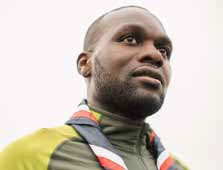
\includegraphics[height=1.5cm]{media/image10}
\par
\vspace{1.4mm}
\fontseries{eb}\linespread{1.2}\selectfont Dwayne Fields\\Scout Ambassador
\par
\vspace{1.2\baselineskip}
\begin{minipage}[t]{\columnwidth}
\fontseries{m}\linespread{1.4}\selectfont
\raggedright
Dwayne is a polar explorer
and speaker. He is the first
black Briton to reach the
North Pole, and only the
second black man in the
world to achieve this feat.
Born in Jamaica, he grew up
in Hackney, London.
\end{minipage}
\vfill
\columnbreak

\includegraphics[height=1.5cm]{media/image11}
\par
\vspace{1.4mm}
\fontseries{eb}\linespread{1.2}\selectfont Helen Glover\\Scout Ambassador
\par
\vspace{1.2\baselineskip}
\begin{minipage}[t]{\columnwidth}
\fontseries{m}\linespread{1.4}\selectfont
\raggedright
Helen is a two-time Olympic
champion and triple World
Champion, winning British
women’s rowing’s first ever
gold medal at London 2012.
\end{minipage}
\vfill
\columnbreak

\includegraphics[height=1.5cm]{media/image9}
\par
\vspace{1.4mm}
\fontseries{eb}\linespread{1.2}\selectfont Tim Peake\\Scout Ambassador
\par
\vspace{1.2\baselineskip}
\begin{minipage}[t]{\columnwidth}
\fontseries{m}\linespread{1.4}\selectfont
\raggedright
ESA Astronaut Major Tim
Peake is also a former Cub
Scout and an advocate of the
power of Scouting to help
young people develop skills
for life.
\end{minipage}
\vfill
\columnbreak
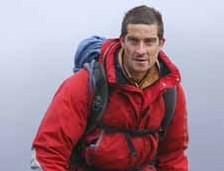
\includegraphics[height=1.5cm]{media/image12}
\par
\vspace{1.4mm}
\fontseries{eb}\linespread{1.2}\selectfont Bear Grylls\\Chief Scout
\par
\vspace{1.2\baselineskip}
\begin{minipage}[t]{\columnwidth}
\fontseries{m}\linespread{1.4}\selectfont
\raggedright
Bear was appointed in 2009
as the youngest ever Chief
Scout of the United Kingdom.
He has inspired hundreds of
thousands of young people
with his positivity, passion for
adventure, courage and
leadership.
\end{minipage}
\vfill
\end{multicols}
\end{minipage}
\hfill
\end{frame}

\changecolours{ScoutPurple}
\section{Thank you} % Attempt to follow Scouts PPTx slide template

\headervisibility
\title{Do~more. Share~more. RGB~more.}
\part{Testing the colours}
%%%%%%%%%%%%%%%%%%%%%%%%%%%%%%%%%%%%%%%%%%%%%%%%%%%%%%%%%%%%%%%%%%%%%
%% Copyright 2020 Mike Jones, <dr.mike.jones@gmail.com>
%% AKA Grey Wolf <mike.jones@mansouthscouts.org>
%% [23rd Manchester (Birch with Fallowfield)]
%% Scout Membership number: 12114313
%
% This file is part of Grey Wolf's Scouts Beamer Theme.
%
% Grey Wolf's Scouts Beamer Theme is free software: you can redistribute
% it and/or modify it under the terms of the GNU General Public License
% as published by the Free Software Foundation, either version 3 of the
% License, or (at your option) any later version.
%
% Grey Wolf's Scouts Beamer Theme is distributed in the hope that it will 
% be useful, but WITHOUT ANY WARRANTY; without even the implied warranty
% of MERCHANTABILITY or FITNESS FOR A PARTICULAR PURPOSE.  See the GNU
% General Public License for more details.
%
% You should have received a copy of the GNU General Public License
% along with Grey Wolf's Scouts Beamer Theme.  If not, see
% <https://www.gnu.org/licenses/>.
%%%%%%%%%%%%%%%%%%%%%%%%%%%%%%%%%%%%%%%%%%%%%%%%%%%%%%%%%%%%%%%%%%%%%

\renewcommand*{\do}[1]{%
\changecolours{#1}%
\section{#1}
\subsection{#1 Subsection}
\frame[allowframebreaks]{\frametitle{#1 Content}\lipsum[1]}
\begin{frame}{Itemize}
\begin{example}
\begin{itemize}
\item First Level 1
\begin{itemize}
\item Second Level 1
\item Second Level 2
\end{itemize}
\item First Level 3
\item First Level 4
\end{itemize}
\end{example}
\end{frame}
\begin{frame}{Enumerate}
\begin{enumerate}
\item 1
\item this is two
\item three
\end{enumerate}
\end{frame}
}
\docsvlist{ScoutScouts, ScoutCubs, ScoutBeavers, ScoutExplorers, ScoutNetwork, ScoutSeaScouts, ScoutAirScouts}       % Basic unit tests with different Scout Colours

\changecolours{ScoutPurple}
\title{Do~more. Share~more. BC~more.}
\part{Recreating the Beamer example Euclid’s Presentation in this theme}
%%%%%%%%%%%%%%%%%%%%%%%%%%%%%%%%%%%%%%%%%%%%%%%%%%%%%%%%%%%%%%%%%%%%%
%% Copyright 2020 Mike Jones, <dr.mike.jones@gmail.com>
%% AKA Grey Wolf <mike.jones@mansouthscouts.org>
%% [23rd Manchester (Birch with Fallowfield)]
%% Scout Membership number: 12114313
%
% This file is part of Grey Wolf's Scouts Beamer Theme.
%
% Grey Wolf's Scouts Beamer Theme is free software: you can redistribute
% it and/or modify it under the terms of the GNU General Public License
% as published by the Free Software Foundation, either version 3 of the
% License, or (at your option) any later version.
%
% Grey Wolf's Scouts Beamer Theme is distributed in the hope that it will 
% be useful, but WITHOUT ANY WARRANTY; without even the implied warranty
% of MERCHANTABILITY or FITNESS FOR A PARTICULAR PURPOSE.  See the GNU
% General Public License for more details.
%
% You should have received a copy of the GNU General Public License
% along with Grey Wolf's Scouts Beamer Theme.  If not, see
% <https://www.gnu.org/licenses/>.
%%%%%%%%%%%%%%%%%%%%%%%%%%%%%%%%%%%%%%%%%%%%%%%%%%%%%%%%%%%%%%%%%%%%%

\changecolours{ScoutPurple}
\section{What Are Prime Numbers?}

\begin{frame}
\frametitle{What Are Prime Numbers?}
\begin{definition}
A \alert{prime number} is a number that has exactly two divisors.
\end{definition}
\end{frame}


\begin{frame}
%\frametitle{What Are Prime Numbers?}
\begin{example}
\begin{itemize}
\item 2 is prime (two divisors: 1 and 2).
  \pause
\item 3 is prime (two divisors: 1 and 3).
  \pause
\item 4 is not prime (\alert{three} divisors: 1, 2, and 4).
\end{itemize}
\end{example}
\end{frame}

\begin{frame}
\frametitle{There Is No Largest Prime Number}
\framesubtitle{The proof uses \textit{reductio ad absurdum}.}
\begin{theorem}
There is no largest prime number.
\end{theorem}
\end{frame}

\begin{frame}
%\frametitle{There Is No Largest Prime Number}
\framesubtitle{The proof uses \textit{reductio ad absurdum}.}
\begin{proof}
\begin{enumerate}
\renewcommand{\theenumi}{\Alph{enumi}}
\item<1-> Suppose $p$ were the largest prime no.
\item<2-> Let $q$ be the product of the first $p$ nos.
\item<3-> Then $q + 1$ is not divisible by any of them.
\item<1-> But $q + 1 > 1$, thus divisible by some prime
number not in the first $p$ nos.\qedhere
\end{enumerate}
\end{proof}
\uncover<4->{The proof used \textit{reductio ad absurdum}.}
\end{frame}

\section{What's Still To Do?}
\subsection{Extra text here}

\begin{frame}
\frametitle{What’s Still To Do?}
\begin{block}{Answered Questions}
How many primes are there?
\end{block}
\begin{block}{Open Questions}
Is every even number the sum of two primes?
\end{block}
\end{frame}

\begin{frame}
\frametitle{What’s Still To Do?}
\begin{columns}
\begin{column}{0.5\textwidth}
\begin{block}{Answered Questions}
How many primes are there?
\end{block}
\end{column}
\column{.5\textwidth}
\begin{block}{Open Questions}
Is every even number the sum of two primes?~\cite{Goldbach1742}
\end{block}
\end{columns}
\end{frame}

\begin{frame}[fragile]
\frametitle{An Algorithm For Finding Prime Numbers.}
\tiny
\begin{verbatim}
int main (void)
{
std::vector<bool> is_prime (100, true);
for (int i = 2; i < 100; i++)
if (is_prime[i])
{
std::cout << i << " ";
for (int j = i; j < 100; is_prime [j] = false, j+=i);
}
return 0;
}
\end{verbatim}
\begin{uncoverenv}<2>
Note the use of \verb|std::|.
\end{uncoverenv}
\end{frame}

\begin{frame}
\frametitle{Further Reading}
\begin{thebibliography}{10}
\bibitem{Goldbach1742}[Goldbach, 1742]
Christian Goldbach.
\newblock A problem we should try to solve before the ISPN '43 deadline,
\newblock \emph{Letter to Leonhard Euler}, 1742.
\end{thebibliography}
\end{frame}
        % Attempt to follow beamer's example setup from manual

\appendix

\title{Do more. Cycle more. Be more.}
\part{Highway Code Example}
\graphicspath{{Motivation/Signs/}{Motivation/Signs/extra/}{Signs/}} % Where are my signs
\logoslide[noheadlogo,type=stacked]
\frame[plain]{\titlepage}
\renewcommand*{\theenumii}{\Alph{enumii}}
{
\bgimage[onlybodyheight,position=l,marginleft=1cm,marginright=2cm,fit=all,alwaysshow]{544}
\twocolframe[rightcol=7cm,leftcol=3cm,title={What is this sign...}]{}{
\large
  \begin{enumerate}[A]
    \item Rope bridge challenge activity ahead
    \item Disco dancers ahead
    \item Zebra crossing ahead
    \item Please remember to step from the moving walkway
  \end{enumerate}
  }
}
{
\bgimage[onlybodyheight,position=l,marginleft=1cm,marginright=2cm,fit=all,alwaysshow]{833-834}
\twocolframe[rightcol=7cm,leftcol=3cm,title={What is this sign...}]{}{
\large
  \begin{enumerate}[A]
    \item Knees bend, arms stretch ra, ra, ra.
    \item Entrance/exit to a car park, private road...
    \item Do the Hokie Cokie
    \item Caution referendums
  \end{enumerate}
  }
}
{
\bgimage[onlybodyheight,position=l,marginleft=1cm,marginright=2cm,fit=all,alwaysshow]{951}
\twocolframe[rightcol=7cm,leftcol=3cm,title={What is this sign...}]{}{
\large
  \begin{enumerate}[A]
    \item Cyclists must carry hula-hoops
    \item Only pedal cycles allowed
    \item Riding of pedal cycles prohibited
    \item Fallowfield loop ahead
  \end{enumerate}
  }
}
{
\bgimage[onlybodyheight,position=l,marginleft=1cm,marginright=2cm,fit=all,alwaysshow]{810}
\twocolframe[rightcol=7cm,leftcol=3cm,title={What is this sign...}]{}{
\large
  \begin{enumerate}[A]
    \item The other way
    \item This way
    \item One-way traffic in direction indicated (sign for pedestrians)
    \item That way
  \end{enumerate}
  }
}
{
\bgimage[onlybodyheight,position=l,marginleft=1cm,marginright=2cm,fit=all,alwaysshow]{2928all}
\twocolframe[rightcol=7cm,leftcol=3cm,title={What is this sign...}]{}{
\large
  \begin{enumerate}[A]
    \item Places beginning with H ahead
    \item Warning, Musicals
    \item County boundary signs
    \item Hurricaneshires
  \end{enumerate}
  }
}
{
\bgimage[onlybodyheight,position=l,marginleft=1cm,marginright=2cm,fit=all,alwaysshow]{562}
\twocolframe[rightcol=7cm,leftcol=3cm,title={What is this sign...}]{}{
\large
  \begin{enumerate}[A]
    \item Pardon Me!
    \item S.P.A.G.
    \item Skittles or bowling
    \item Other danger ahead. Plate beneath indicates the nature of the hazard
  \end{enumerate}
  }
}
{
\bgimage[onlybodyheight,position=l,marginleft=1cm,marginright=2cm,fit=all,alwaysshow]{957}
\twocolframe[rightcol=7cm,leftcol=3cm,title={What is this sign...}]{}{
\large
  \begin{enumerate}[A]
    \item Bike cupboards on your left
    \item You must leave your bike here and carry on on-foot
    \item Bike pole vaulting contest here
    \item Route comprising a separated track and path for cycles and pedestrians
  \end{enumerate}
  }
}
{
\bgimage[onlybodyheight,position=l,marginleft=1cm,marginright=2cm,fit=all,alwaysshow]{953.1V}
\twocolframe[rightcol=7cm,leftcol=3cm,title={What is this sign...}]{}{
\large
  \begin{enumerate}[A]
    \item Buses are heavier that trams
    \item Vehicle piggy-back zone
    \item Trams are lighter than buses
    \item Route for use by buses and tramcars only
  \end{enumerate}
  }
}
{
\bgimage[onlybodyheight,position=l,marginleft=1cm,marginright=2cm,fit=all,alwaysshow]{522}
\twocolframe[rightcol=7cm,leftcol=3cm,title={What is this sign...}]{}{
\large
  \begin{enumerate}[A]
    \item It wasn't me
    \item Tweedledum
    \item Two-way traffic on route crossing ahead
    \item Tweedledee
  \end{enumerate}
  }
}
{
\bgimage[onlybodyheight,position=l,marginleft=1cm,marginright=2cm,fit=all,alwaysshow]{827.2}
\twocolframe[rightcol=7cm,leftcol=3cm,title={What is this sign...}]{}{
\large
  \begin{enumerate}[A]
    \item Helicopters ahead
    \item Hospital ahead with accident and emergency facilities
    \item Warning big letter 'H' ahead
    \item Hospital with accident and emergency dept
  \end{enumerate}
  }
}
{
\bgimage[onlybodyheight,position=l,marginleft=1cm,marginright=2cm,fit=all,alwaysshow]{7001}
\twocolframe[rightcol=7cm,leftcol=3cm,title={What is this sign...}]{}{
\large
  \begin{enumerate}[A]
    \item Triangles ahead
    \item Look, your left shoelace is undone
    \item Caution elephant poo
    \item Road works or temporary obstruction of the carriageway ahead
  \end{enumerate}
  }
}
{
\bgimage[onlybodyheight,position=l,marginleft=1cm,marginright=2cm,fit=all,alwaysshow]{T201}
\twocolframe[rightcol=7cm,leftcol=3cm,title={What is this sign...}]{}{
\large
  \begin{enumerate}[A]
    \item Welcome to Lancashire
    \item Garden centre
    \item Mmmm, Cadbury's roses
    \item Tourist symbol for England only: Tourist attraction recognised by a regional tourist board or the English Tourist Board
  \end{enumerate}
  }
}
{
\bgimage[onlybodyheight,position=l,marginleft=1cm,marginright=2cm,fit=all,alwaysshow]{2602.2-66_ii}
\twocolframe[rightcol=7cm,leftcol=3cm,title={What is this sign...}]{}{
\large
  \begin{enumerate}[A]
    \item Road limited to 66 bicycles at a time
    \item Follow these signs to get to Los Angeles
    \item Rock'n'roll music reference ahead
    \item A national cycle network route that follows the Rochdale canal to Leeds and beyond
  \end{enumerate}
  }
}
{
\bgimage[onlybodyheight,position=l,marginleft=1cm,marginright=2cm,fit=all,alwaysshow]{501}
\twocolframe[rightcol=7cm,leftcol=3cm,title={What is this sign...}]{}{
\large
  \begin{enumerate}[A]
    \item Junction ahead controlled by a STOP or GIVE WAY sign
    \item Sign thieves operate here
    \item Um, something might be upside down (again)
    \item White cats in snow
  \end{enumerate}
  }
}
{
\bgimage[onlybodyheight,position=l,marginleft=1cm,marginright=2cm,fit=all,alwaysshow]{555}
\twocolframe[rightcol=7cm,leftcol=3cm,title={What is this sign...}]{}{
\large
  \begin{enumerate}[A]
    \item Always park on the wobbly lines
    \item Watch out for large jelly-fish
    \item Dip your headlights
    \item Quayside or river bank ahead
  \end{enumerate}
  }
}
{
\bgimage[onlybodyheight,position=l,marginleft=1cm,marginright=2cm,fit=all,alwaysshow]{670V20}
\twocolframe[rightcol=7cm,leftcol=3cm,title={What is this sign...}]{}{
\large
  \begin{enumerate}[A]
    \item Minimum speed 20 mph
    \item 20 points if you hit this sign
    \item Happy birthday to you
    \item Maximum speed limit of 20 miles per hour
  \end{enumerate}
  }
}
{
\bgimage[onlybodyheight,position=l,marginleft=1cm,marginright=2cm,fit=all,alwaysshow]{2603}
\twocolframe[rightcol=7cm,leftcol=3cm,title={What is this sign...}]{}{
\large
  \begin{enumerate}[A]
    \item Junction ahead leading to a parking place for pedal cycles
    \item Bicycles being chased by large letter P's must go upwards here.
    \item Picycles over there
    \item Toilet but only for cyclists
  \end{enumerate}
  }
}
{
\bgimage[onlybodyheight,position=l,marginleft=1cm,marginright=2cm,fit=all,alwaysshow]{552}
\twocolframe[rightcol=7cm,leftcol=3cm,title={What is this sign...}]{}{
\large
  \begin{enumerate}[A]
    \item \mbox{Cat-at-at-at-tt-le-le gri-d-d-d-d} ahead, too late!
    \item No barbeques here
    \item Caution ankle twisters
    \item Cattle grid ahead
  \end{enumerate}
  }
}
{
\bgimage[onlybodyheight,position=l,marginleft=1cm,marginright=2cm,fit=all,alwaysshow]{551.2}
\twocolframe[rightcol=7cm,leftcol=3cm,title={What is this sign...}]{}{
\large
  \begin{enumerate}[A]
    \item Duck! Beaver paper aeroplane testing zone
    \item Foul! Hand-ball
    \item Frogs?
    \item Wild fowl likely to be in road ahead
  \end{enumerate}
  }
}
{
\bgimage[onlybodyheight,position=l,marginleft=1cm,marginright=2cm,fit=all,alwaysshow]{512}
\twocolframe[rightcol=7cm,leftcol=3cm,title={What is this sign...}]{}{
\large
  \begin{enumerate}[A]
    \item Bend ahead to the right
    \item Bow to the scout leader on the right
    \item We open at ten past six
    \item Low flying boomerangs
  \end{enumerate}
  }
}
{
\bgimage[onlybodyheight,position=l,marginleft=1cm,marginright=2cm,fit=all,alwaysshow]{770}
\twocolframe[rightcol=7cm,leftcol=3cm,title={What is this sign...}]{}{
\large
  \begin{enumerate}[A]
    \item Level crossing with gate or barrier ahead
    \item Window cleaner has fallen over
    \item Caution, escaped zoo animals
    \item Caution fencing ahead
  \end{enumerate}
  }
}
{
\bgimage[onlybodyheight,position=l,marginleft=1cm,marginright=2cm,fit=all,alwaysshow]{520}
\twocolframe[rightcol=7cm,leftcol=3cm,title={What is this sign...}]{}{
\large
  \begin{enumerate}[A]
    \item Divining rods at the ready
    \item Tune your engine
    \item Caution the letter 'Y' has fallen over
    \item Dual carriageway ends ahead
  \end{enumerate}
  }
}
{
\bgimage[onlybodyheight,position=l,marginleft=1cm,marginright=2cm,fit=all,alwaysshow]{2702}
\twocolframe[rightcol=7cm,leftcol=3cm,title={What is this sign...}]{}{
\large
  \begin{enumerate}[A]
    \item The bridge is down quick go right, go right I tell you!
    \item Procrastination
    \item Start of temporary diversion route to the right
    \item Look a squirrel
  \end{enumerate}
  }
}
{
\bgimage[onlybodyheight,position=l,marginleft=1cm,marginright=2cm,fit=all,alwaysshow]{956}
\twocolframe[rightcol=7cm,leftcol=3cm,title={What is this sign...}]{}{
\large
  \begin{enumerate}[A]
    \item It will be raining bikes later
    \item Hold hands with your adult while they think about bikes
    \item Route for use by pedal cycles and pedestrians only
    \item Gosh isn't that bike big?
  \end{enumerate}
  }
}
{
\bgimage[onlybodyheight,position=l,marginleft=1cm,marginright=2cm,fit=all,alwaysshow]{4003.7}
\twocolframe[rightcol=7cm,leftcol=3cm,title={What is this sign...}]{}{
\large
  \begin{enumerate}[A]
    \item A can I press it button A toucan crossing button
    \item Near side light signals and instructions for pedestrians and cyclists at a Toucan crossing
    \item A red herring crossing button
    \item A zebra crossing beacon
  \end{enumerate}
  }
}
{
\bgimage[onlybodyheight,position=l,marginleft=1cm,marginright=2cm,fit=all,alwaysshow]{950}
\twocolframe[rightcol=7cm,leftcol=3cm,title={What is this sign...}]{}{
\large
  \begin{enumerate}[A]
    \item Only bicycles with triangular wheels allowed
    \item Cycle route ahead warning
    \item Cyclists must wear a wizards hat at all times
    \item Cyclists must carry a hazard warning triangle
  \end{enumerate}
  }
}

\section{That's all folks!}
\frame{The images in this presentation are Crown Copyright and are licenced for use in this scout quiz context.}

\end{document}
